%----------------------------------------------------------------------------------------
%	PACKAGES & THEMES
%----------------------------------------------------------------------------------------

\documentclass[8pt]{beamer}

\usepackage{etex}
\mode<presentation> {
\usetheme{Vilanova}
}

\usepackage[french]{babel}
\usepackage[utf8]{inputenc}
\usepackage{array}
\usepackage{graphicx}
\usepackage{booktabs}
\usepackage{amsmath,amssymb,amsthm}
\usepackage{xcolor}
\usepackage{tikz}
\usetikzlibrary{arrows}
\usepackage{pifont}
\usepackage{listings,color}
\usepackage{xmpmulti}

\definecolor{listcomment}{rgb}{0.0,0.5,0.0}
\definecolor{listkeyword}{rgb}{0.0,0.0,0.5}
\definecolor{listnumbers}{gray}{0.65}
\definecolor{listlightgray}{gray}{0.955}
\definecolor{listwhite}{gray}{1.0}

\AtBeginSection[]
{
\addtocounter{framenumber}{-1}
\begin{frame}
\frametitle{Sommaire}
\tableofcontents[currentsection]
\end{frame}}

%----------------------------------------------------------------------------------------
%	PAGE TITRE
%----------------------------------------------------------------------------------------
\title{Orfeo ToolBox}
\subtitle{Traitement d'images et télédétection: quoi de neuf dans Orfeo ToolBox ?}
\author{Équipe OTB}% date and event here
\date{FOSS4G-FR 2018}

\pgfdeclareimage[height=96mm,width=128mm]{background}{images/fondsClairSansLogo}
\pgfdeclareimage[height=0.2cm]{cc}{images/CC-licence.png}
\setbeamertemplate{background}{\pgfuseimage{background}}
\pgfdeclareimage[height=0.6cm]{logoIncrust}{images/logoIncrust}
\pgfdeclareimage[height=0.6cm]{OSGeo_logo}{images/OSGeo_logo}
\logo{
\begin{tabular}{p{0.22\textwidth}p{0.58\textwidth}p{0.1\textwidth}p{0.1\textwidth}}
\href{http://www.osgeo.org}{\pgfuseimage{OSGeo_logo}}
& \vspace{-0.03\textwidth} \scriptsize{} % date and event here
& \href{http://creativecommons.org/licenses/by-sa/3.0/}{\pgfuseimage{cc}} & \href{http://www.orfeo-toolbox.org}{\pgfuseimage{logoIncrust}}\\
\end{tabular}
}

\titlegraphic{\vspace*{-5em}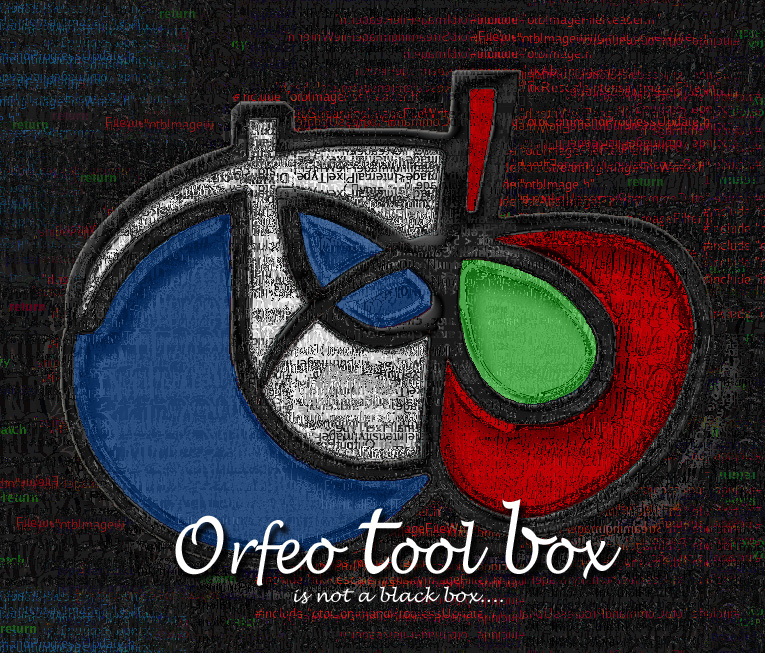
\includegraphics[width=.4\textwidth]{images/LOGOTB_blackbox.png}}

\begin{document}
\begin{frame}
\titlepage
\end{frame}

\section*{Introduction}

\begin{frame}
\frametitle{Si vous ne retenez qu'une planche\ldots}
\begin{block}{L'Orfeo ToolBox est:}
\begin{itemize}
\item Une \textbf{bibliothèque de traitement d'images} pour la télédétection
\item \textbf{Un logiciel libre} diffusé sous licence Apache v2.0 (depuis OTB 6.0, précédemment CeCILL-v2)
\item \textbf{Financée et développée par le CNES} principalement 
\item \alert{CNES sponsor Or FOSS4G-FR 2018!}
\item Écrite en \textbf{C++} sur la base d'\href{www.itk.org}{ITK} (imagerie médicale)
\item Construite sur les épaules de géants (ITK, GDAL, OSSIM, OpenCV\ldots)
\item Conçue pour traiter de \textbf{gros volumes de données} de manière transparente grâce au traitement par morceaux et à la parallélisation
\item \alert{Logiciel officiel OSGeo depuis 2017!}
\end{itemize}
\end{block}

\begin{center}
{\huge\textcolor{red}{\href{http://www.orfeo-toolbox.org}{orfeo-toolbox.org}}}
\end{center}

\end{frame}

\begin{frame}
\frametitle{Pourquoi un logiciel libre ?}

\begin{block}{Diffusion maximale}
L'OTB est un logiciel à destination de tous les utilisateurs d'imagerie
spatiale. Sa diffusion large contribue au rayonnement des missions (Pléiades, Sentinels\ldots)
\end{block}

\begin{block}{Qualité et efficacité}
Le domaine fonctionnel de l'OTB est vaste, son développement nécessite du temps
et de l'expertise. L'ouverture des sources favorise:
\begin{itemize}
\item L'appropriation et la validation par la communauté des utilisateurs,
\item Les contributions et les corrections de bugs par les utilisateurs,
\item La dissémination sur de multiples plateformes.
\end{itemize}
\end{block}

\begin{block}{Démarche scientifique}
L'OTB capitalise une partie de la R\&D du CNES en extraction d'information, l'ouverture des sources permet une démarche de \textbf{recherche reproductible}.
\end{block}

\end{frame}

\section{Fonctionnalités}

%% \begin{frame}
%% \frametitle{Les grandes familles de fonctionnalités dans l'OTB (forcément incomplètes)}

%% \begin{block}{Pré-traitements}
%% \begin{itemize}
%% \item Calibration radiométrique, ortho-rectification, reprojection (raster et vecteur), pan-sharpening, stéréo-rectification,
%% \item Capteurs supportés: Sentinels, Pléiades, SPOT6, SPOT5, capteurs DigitalGlobe
%% \item Modélisation géométrique fournie par OSSIM, support de MNT SRTM ou GeoTIFF
%% \end{itemize}
%% \end{block}

%% \begin{block}{Manipulation d'images et de vecteurs}
%% \begin{itemize}
%% \item Formats supportés par Gdal (raster et vecteur), conversion raster/vecteur
%% \item Extraction de ROI, de bandes spectrales, concaténation ou séparation des bandes spectrales,
%% \item calcul mathématiques entre bandes, color mapping, optimisation du contraste
%% \item Filtrage linéaire, morphologie mathématique,
%% \end{itemize}
%% \end{block}
%% \end{frame}

%% \begin{frame}
%% \frametitle{Les grandes familles de fonctionnalités dans l'OTB (forcément incomplète)}

%% \begin{block}{Détection d'éléments saillants et calcul de primitives}
%% \begin{itemize}
%% \item Détection de contours, points d'intérêt SIFT et SURF, lignes, angles droits
%% \item Indices radiométriques, indices de textures (Haralick, SFS, PanTex)
%% \item Descripteurs statistiques locaux (moments de Flusser, HOG)
%% \item Matching de points d'intérêts
%% \end{itemize}
%% \end{block}

%% \begin{block}{Détection de changement}
%% \begin{itemize}
%% \item Algorithme classique avec métrique de comparaison d'images,
%% \item Algorithme MAD (Multivariate Alteration Detector)
%% \end{itemize}
%% \end{block}

%% \begin{block}{Réduction de la dimension, traitement hyperspectraux}
%% \begin{itemize}
%% \item Réduction de la dimension: PCA, NAPCA, ICA, MAF \ldots
%% \item Estimation de la dimension et extraction des pixels purs: algorithme VCA
%% \end{itemize}
%% \end{block}

%% \end{frame}

%% \begin{frame}
%% \frametitle{Les grandes familles de fonctionnalités dans l'OTB (forcément incomplète)}
%% \begin{block}{Segmentation}
%% \begin{itemize}
%% \item Algorithmes de segmentation Connected Components, MeanShift, Ligne de partage des eaux
%% \item Méthodologie pour une application large échelle,
%% \item Représentation vectorielles et raster des résultats, avec capacités d'analyse objet
%% \end{itemize}
%% \end{block}

%% \begin{block}{Classification}
%% \begin{itemize}
%% \item Supervision et classification d'images avec 9 algorithmes au choix (dont SVM et forêts aléatoires)
%% \item Fusion et régularisation de cartes de classification
%% \item Clustering de type K-Means ou carte de Kogonen
%% \item Classification objets (segments issus d'une segmentation)
%% \end{itemize}
%% \end{block}

%% \end{frame}

\vspace*{-6.5mm}
\begin{frame}[plain]
\hspace*{-11mm}
    \includegraphics[keepaspectratio,height=1.1\paperheight]{images/mayotte2012.png}
\end{frame}

\vspace*{-6.5mm}
\begin{frame}[plain]
\hspace*{-11mm}
    \includegraphics[keepaspectratio,height=1.1\paperheight]{images/mayotte2013.png}
\end{frame}

\vspace*{-6.5mm}
\begin{frame}[plain]
\hspace*{-11mm}
    \includegraphics[keepaspectratio,height=1.1\paperheight]{images/mayotte_mad.png}
\end{frame}

\vspace*{-6.5mm}
\begin{frame}[plain]
\hspace*{-11mm}
\includegraphics[keepaspectratio,height=1.1\paperheight]{images/saint_paul_lsd.png}
\end{frame}

\vspace*{-6.5mm}
\begin{frame}[plain]
\hspace*{-11mm}
    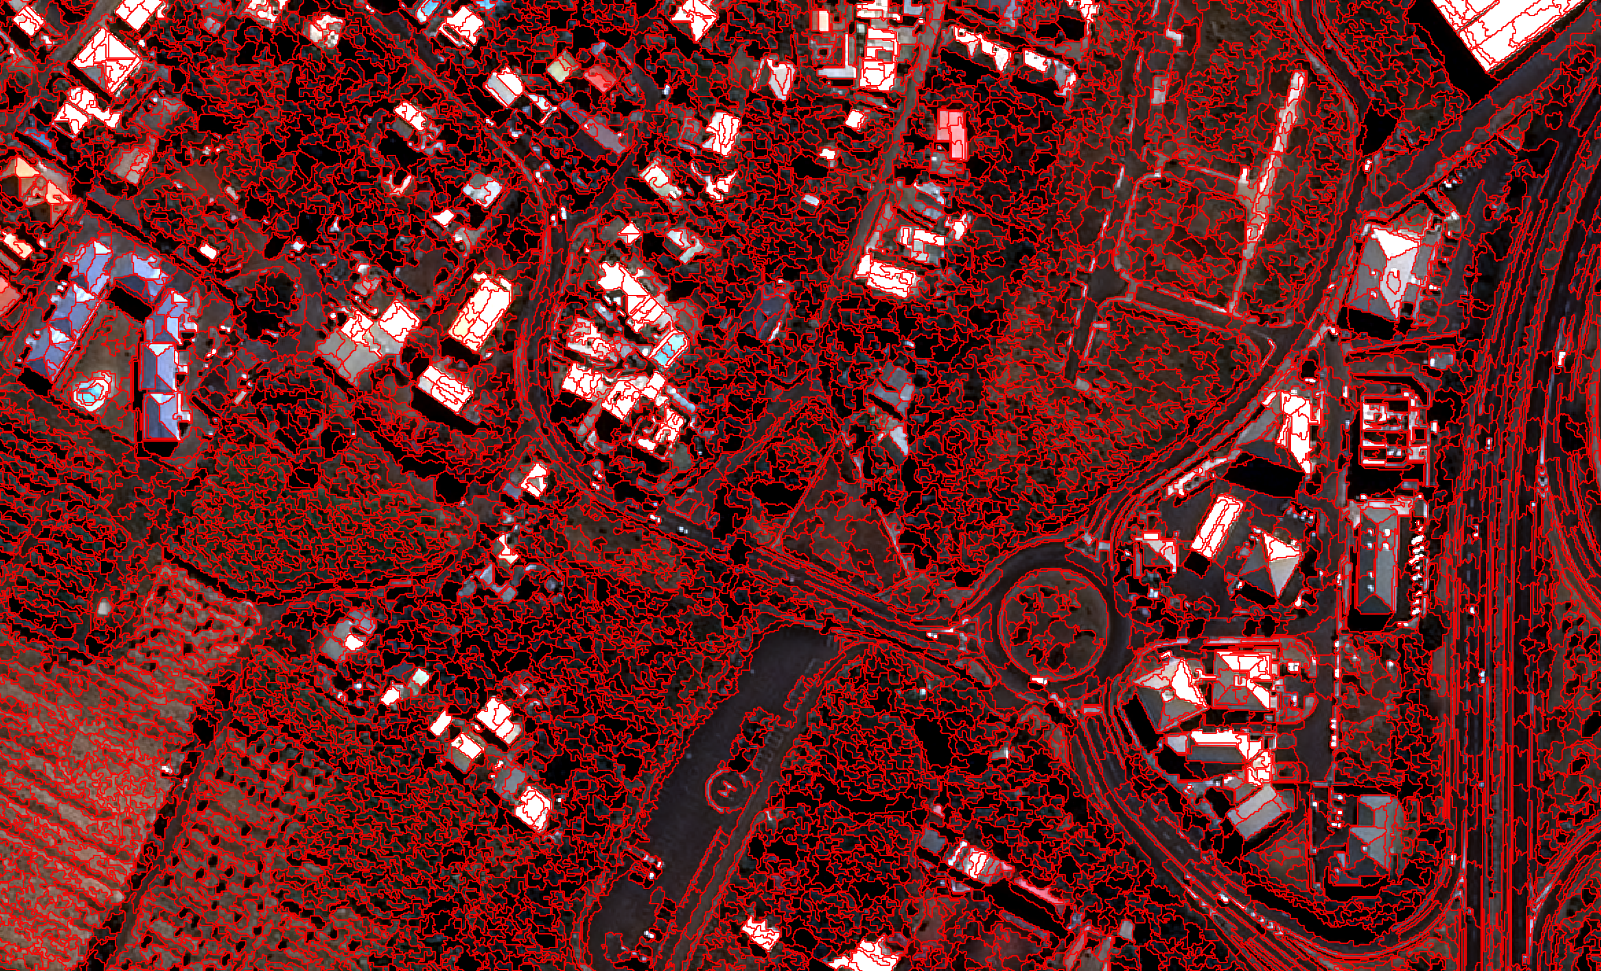
\includegraphics[keepaspectratio,height=1.1\paperheight]{images/segmentation.png}
\end{frame}

\vspace*{-6.5mm}
\begin{frame}[plain]
\hspace*{-11mm}
    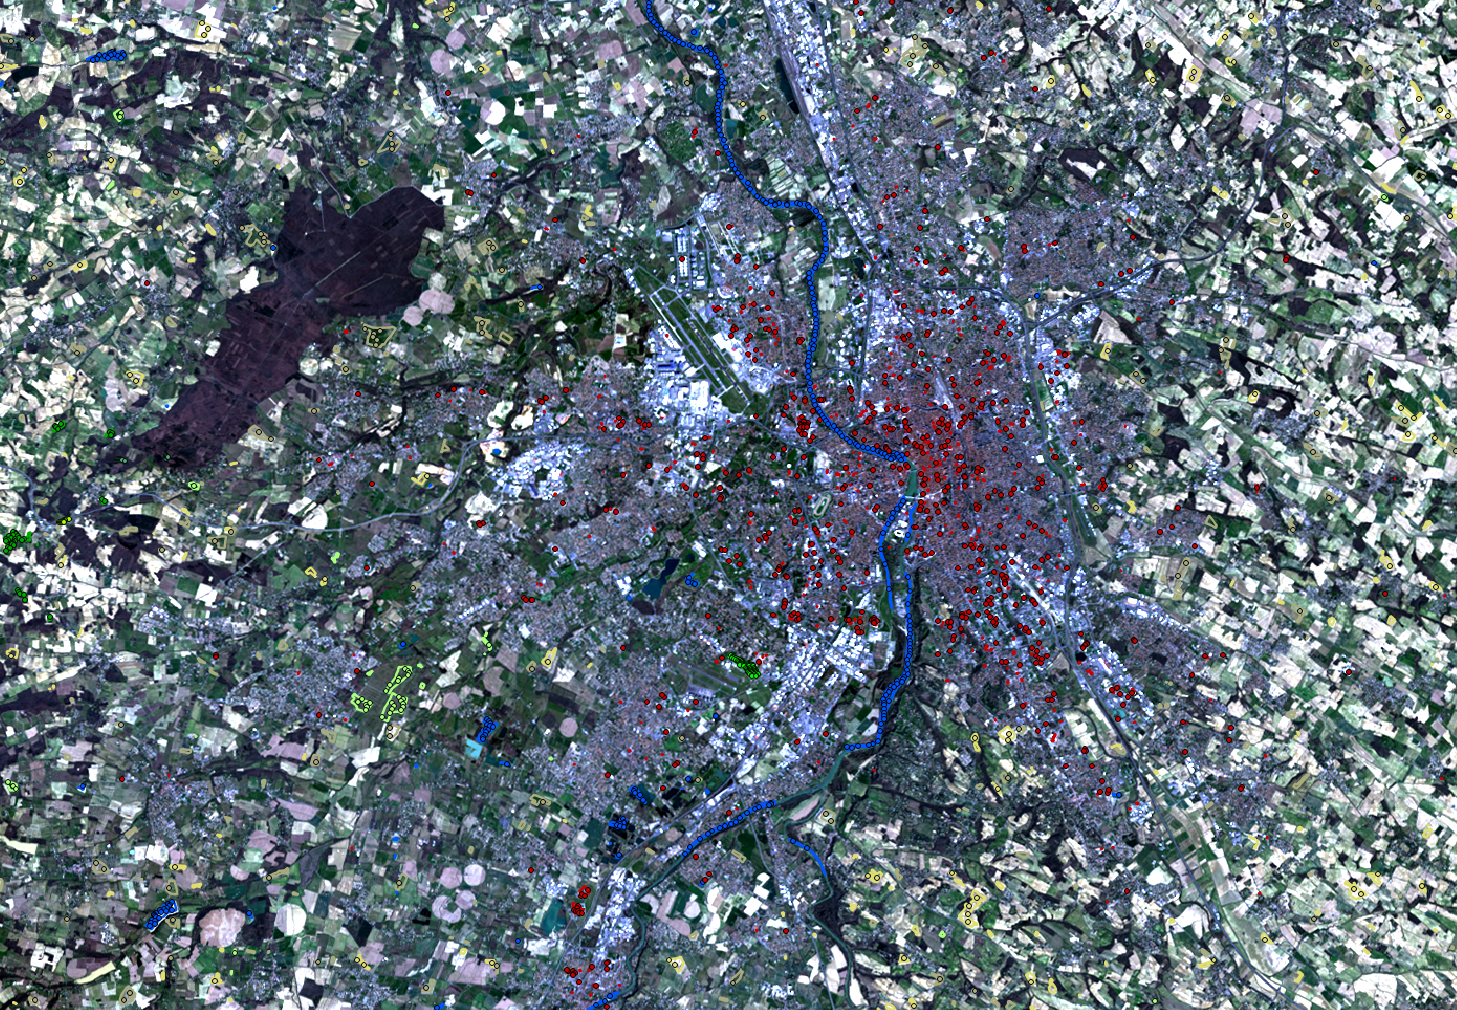
\includegraphics[keepaspectratio,height=1.1\paperheight]{../../Courses/org/WorkshopGuide/Images/samples_selection.png}
\end{frame}


\vspace*{-6.5mm}
\begin{frame}[plain]
\hspace*{-11mm}
    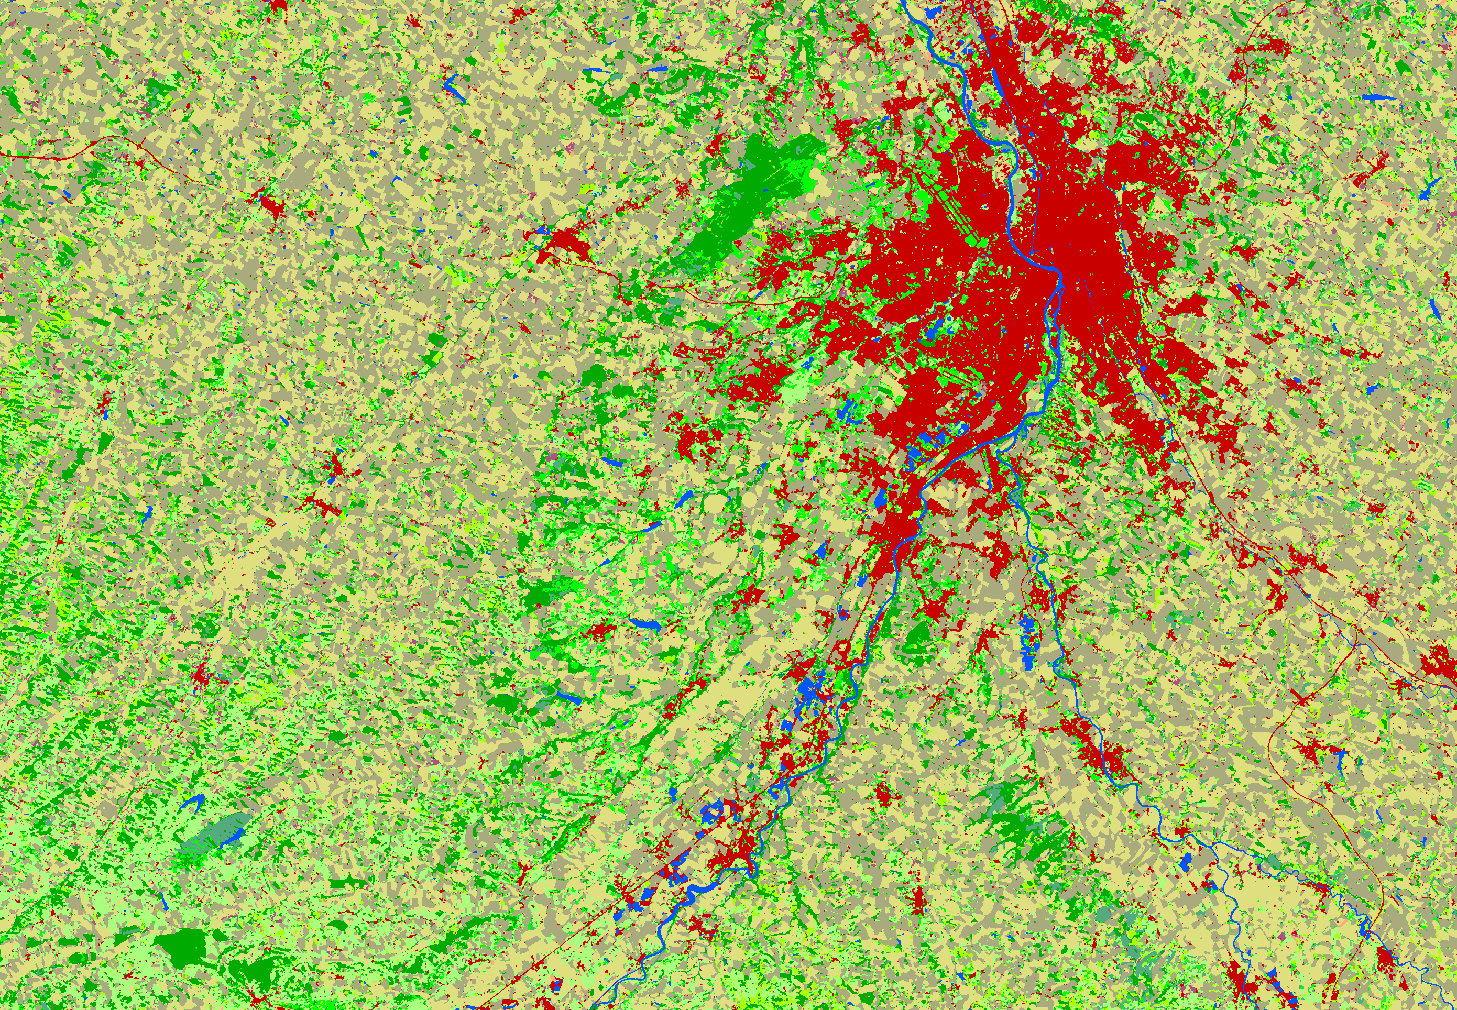
\includegraphics[keepaspectratio,height=1.1\paperheight]{../../Courses/org/WorkshopGuide/Images/final_classification.png}
\end{frame}

\vspace*{-6.5mm}
\begin{frame}[plain]
\hspace*{-11mm}
    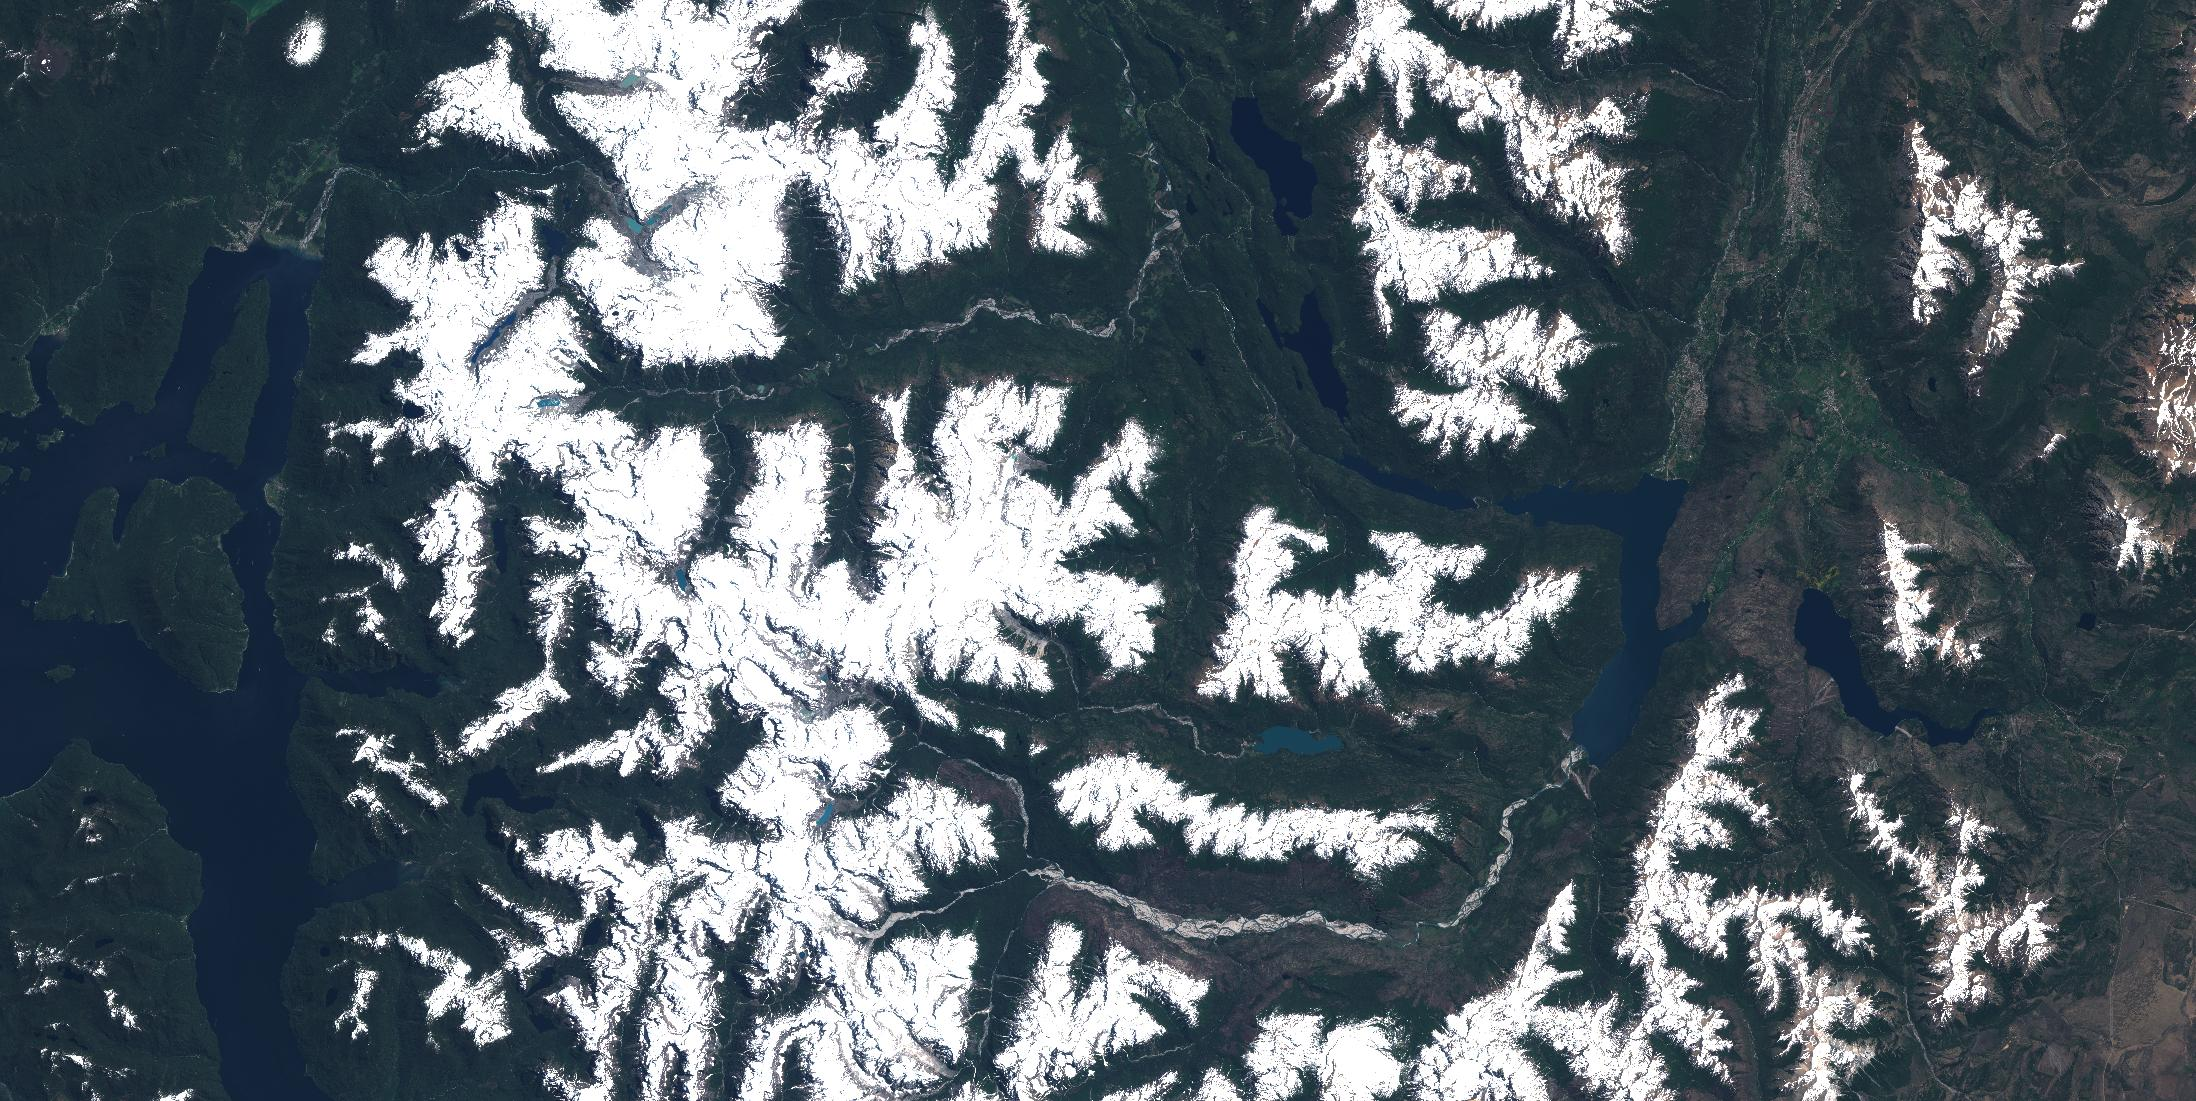
\includegraphics[keepaspectratio,height=1.1\paperheight]{images/imag4tci.jpg}
\end{frame}

\vspace*{-6.5mm}
\begin{frame}[plain]
\hspace*{-11mm}
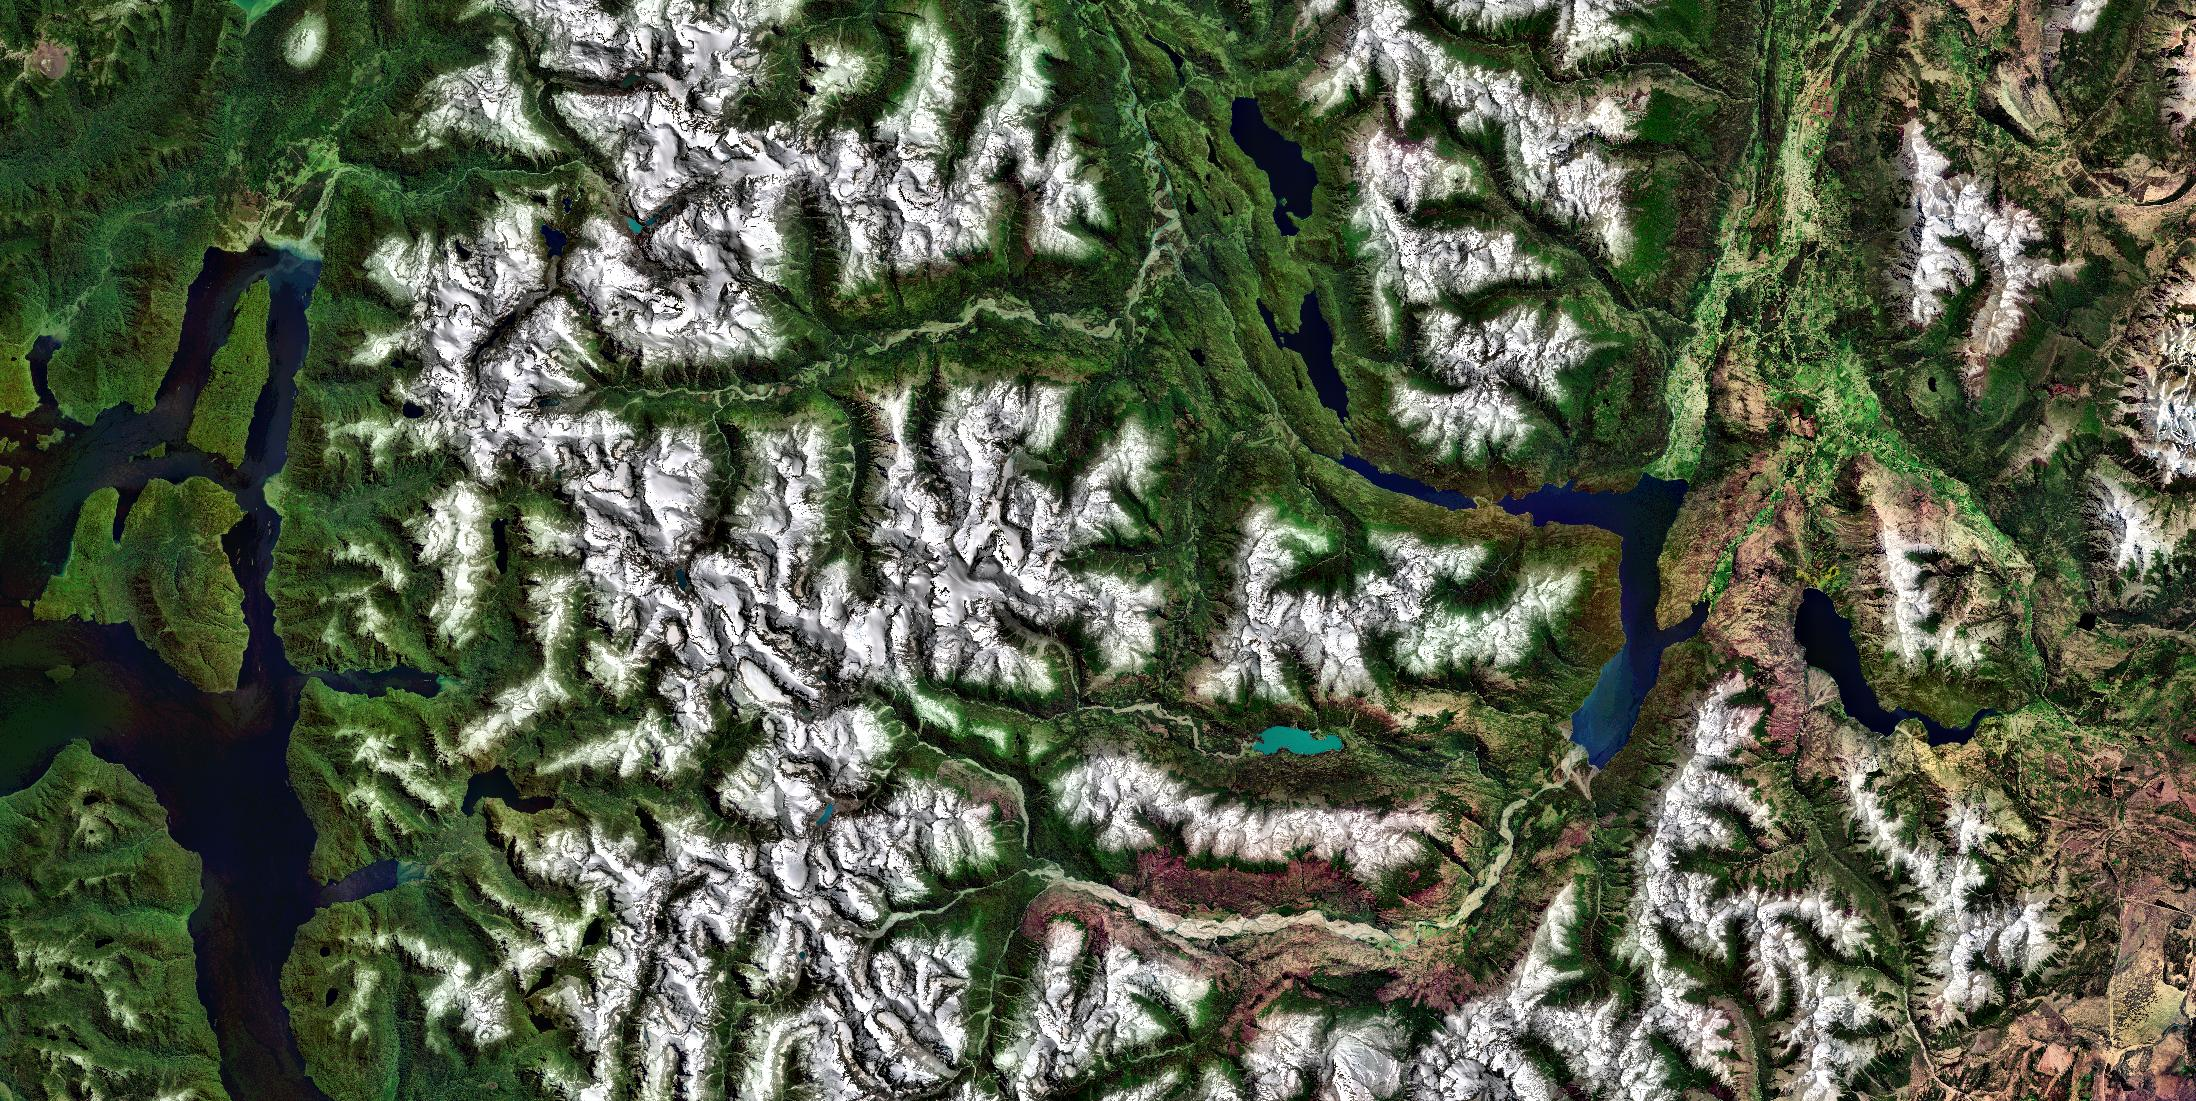
\includegraphics[keepaspectratio,height=1.1\paperheight]{images/image4_glob_each_lim20_8b_sub.jpg}
\end{frame}

\section{Caractéristiques clés}

\begin{frame}
\frametitle{Construite sur des logiciels libres tiers performants}
\begin{block}{Motivations}
\begin{itemize}
\item A chaque fois que c'est possible, l'Orfeo ToolBox s'appuie sur des
  logiciels libres existants
\item Cette position d'intégrateur permet d'accroître rapidement le nombre de fonctions tout en assurant leurs validité
\item Elle permet également de créer de nouvelles fonctionnalités par hybridation
\end{itemize}
\end{block}

\begin{block}{Les logiciels tiers principaux}
\begin{itemize}
\item \href{www.itk.org}{ITK}: modélisation de la chaîne de traitement
\item \href{www.gdal.org}{GDAL}: accès aux données images et vecteurs,
\item \href{www.ossim.org}{OSSIM}: modélisation géométrique des prises de vues,
\item \href{www.opencv.org}{OpenCV} et \href{www.libsvm.org}{LibSVM}: fonctionnalités de classification supervisée,
\item \href{www.muparser.org}{MuParser} et \href{www.muparserx.org}{MuParserX}:
analyse dynamique d'expressions mathématiques.
\end{itemize}
\end{block}


\end{frame}

\begin{frame}
\frametitle{Compatible (et disponible) pour un maximum de plateformes}
\begin{columns}
\column{0.5\textwidth}
\begin{block}{Objectif multi-plateforme}
\begin{itemize}
\item Compiler avec les versions récentes de:
\begin{itemize}
\item GCC
\item Clang
\item MinGW
\item Visual Studio\ldots
\end{itemize}
\item Des paquets binaires sont disponibles en fonction de la plateforme:
\begin{itemize}
\item Dépôt UbuntuGIS pour Ubuntu,
\item Intégration à OSGeo4W et paquets indépendants pour Windows,
\item Paquets MacPort, formule HomeBrew et image dmg pour Mac OS X\ldots
\end{itemize}
\end{itemize}
\end{block}
\column{0.5\textwidth}
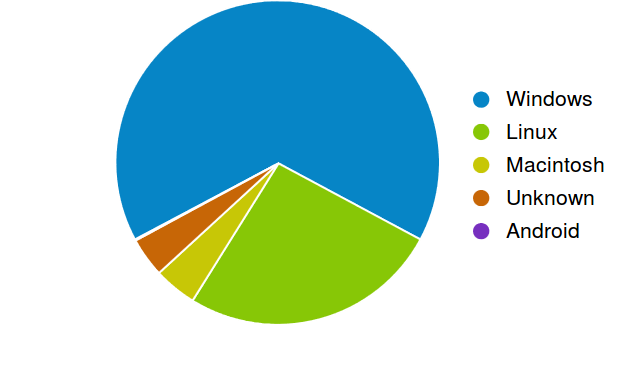
\includegraphics[width=\textwidth]{images/OTB4_download_sourceforge_os_crop.png}
\begin{center}
\tiny{Système d'exploitation des téléchargements sur Sourceforge (ne tient pas compte des autres dépôt)}
\end{center}
\end{columns}
\end{frame}

\begin{frame}
\frametitle{Flexibilité, passage à l'échelle: \textit{Pipeline}, \textit{Streaming} et \textit{multithreading}}

\begin{block}{Le modèle de \textit{Pipeline}}
\begin{center}
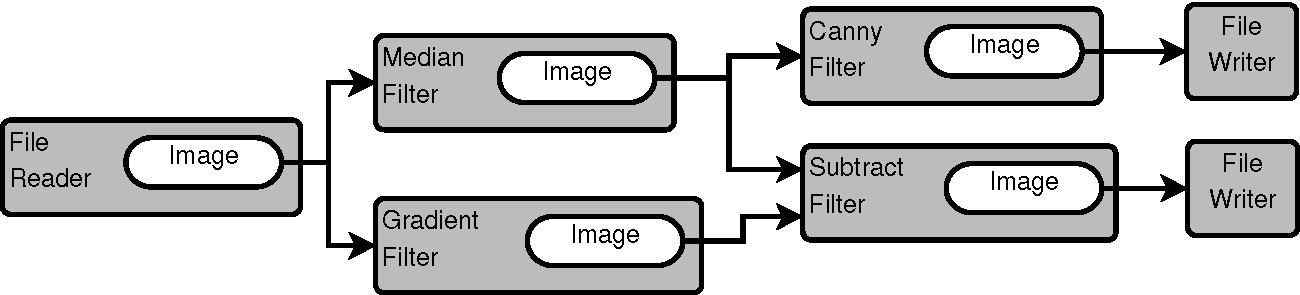
\includegraphics[width=0.7\textwidth]{images/ProcessObjectDataObject.png}
\end{center}
\end{block}
\vspace{-0.5cm}
\begin{block}{\textit{Streaming}}
\begin{center}
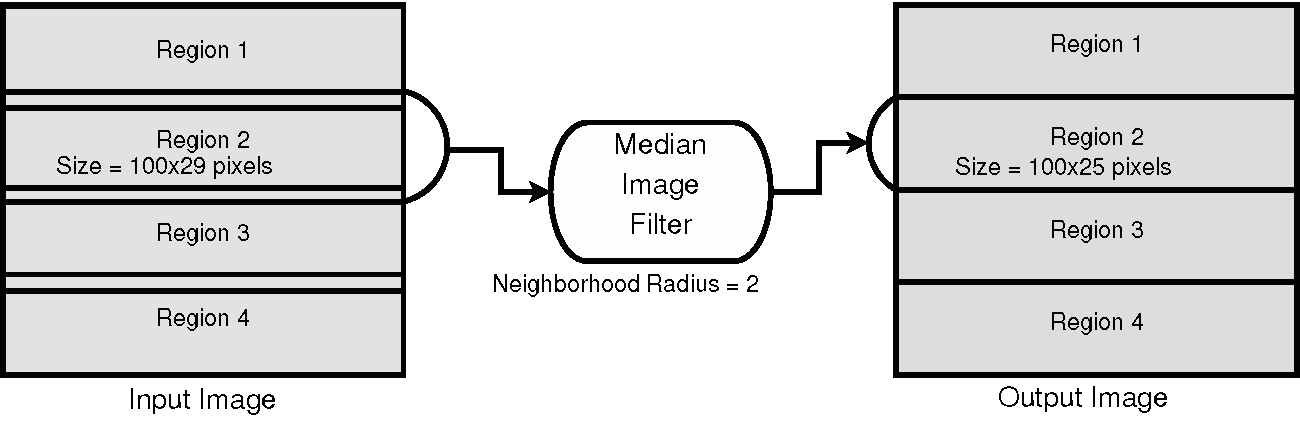
\includegraphics[width=0.7\textwidth]{images/StreamingImageDiagram.png}
\end{center}
\end{block}
\vspace{-0.5cm}
\begin{center}
\tiny{source: http://www.aosabook.org/en/itk.html}
\end{center}
\end{frame}

\begin{frame}
  \frametitle{Projets et logiciels utilisant l'OTB}
  \vspace{-0.5cm}
\begin{columns}
  \column{0.55\textwidth}
  \begin{itemize}
    \item QGIS processing, Zoo-Project...
    \item Certains composant des segments sols S2 et
      Venus (CNES et ESA)
    \item Logiciel éducatif Terr'Image
    \item Produits l'échelle nationale en France
      dans THEIA (Occupation du sol, masques de neige, et même produits 2A...)
    \item Projet ESA S2 for Agriculture
    \item Logiciel Gnorasi (National Technical University of Athens)
    \item Projet GEOSUD (IRSTEA)
    \item Programme de recherche TCM (ETS Quebec)
    \item Chaînes de traitement: au CEREMA,au SERTIT...
  \end{itemize}
  \column{0.6\textwidth}
\begin{center}
  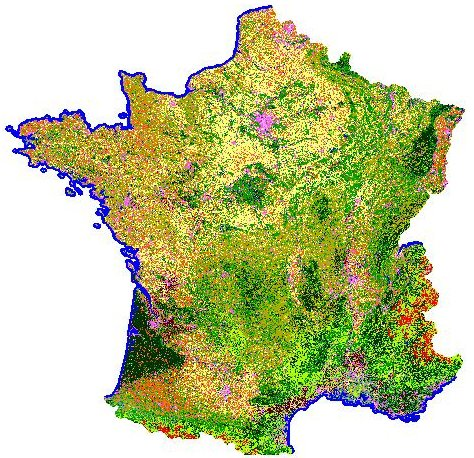
\includegraphics[width=0.6\textwidth,height=0.35\textheight]{images/oso-2017.jpeg}\\
  \tiny{Occupation du sol(2017-CESBIO)}
  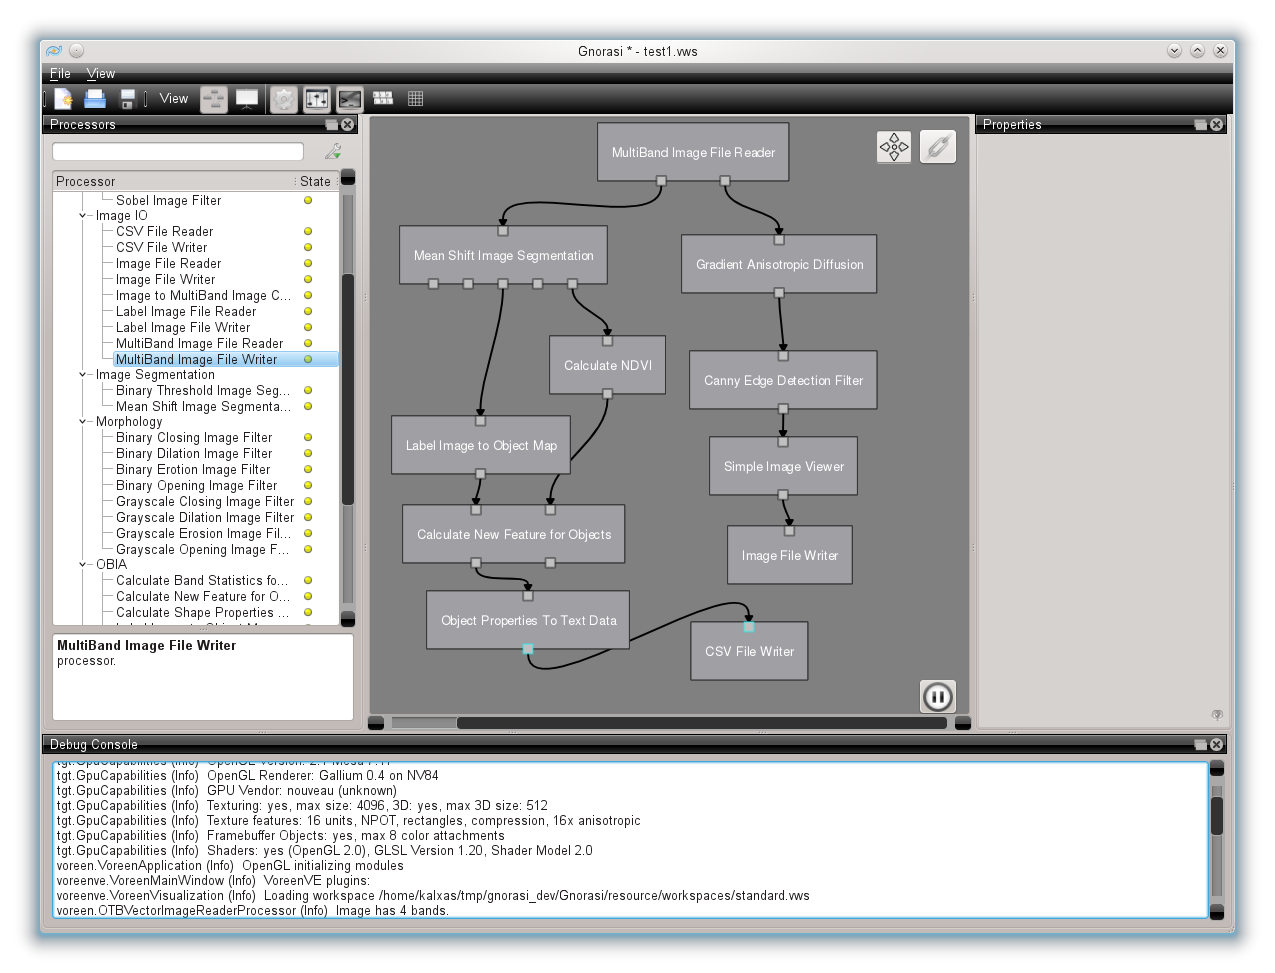
\includegraphics[width=0.6\textwidth]{images/gnorasi2.png}\\
  \tiny{Interface logiciel Gnorasi}
\end{center}
\end{columns}
\end{frame}

\section{Comment utiliser OTB?}

\begin{frame}
\frametitle{Comment utiliser l'OTB?}
\vspace{-0.5cm}
\begin{center}
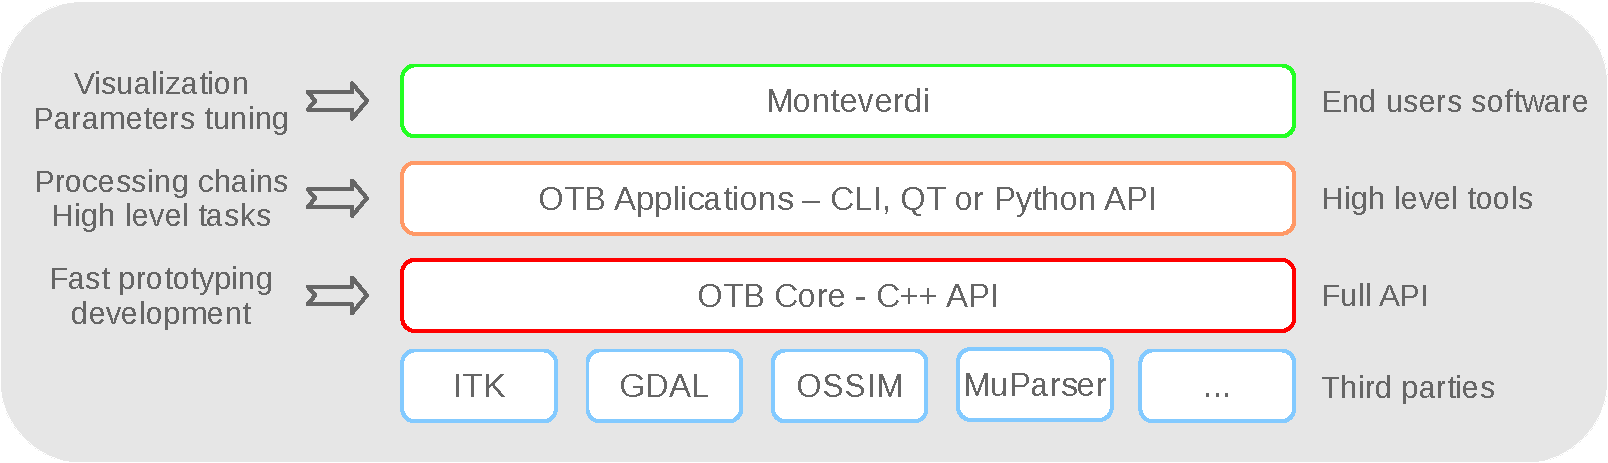
\includegraphics[width=\textwidth]{images/sandwich.pdf}
\end{center}
\vspace{-0.5cm}
\begin{block}{Écrire son propre code}
 Flexible, accès à l'API complète, demande une connaissance en C++
\end{block}
\begin{block}{Utiliser les applications}
 Fonctions de haut niveau (par ex. segmentation), appel en ligne de commande, via une interface graphique, ou depuis Python. Peut être étendue (création d'applications)
\end{block}
\begin{block}{Utiliser Monteverdi}
Visualisation, gestion persistante des données, \textcolor{red}{Accès à l'ensemble des applications}
\end{block}
\end{frame}

\begin{frame}
\frametitle{Les applications: codées une fois, utilisables partout}
\begin{columns}
\column{0.5\textwidth}
\begin{itemize}
\item 87 applications sont livrées avec l'OTB
\item 1 application $=$ 1 librairie dynamique (plugin)
\item Les applications sont auto-descriptives et auto-documentées
\item Les applications peuvent être étendues en dehors de l'OTB
\item Plusieurs interfaces sont disponibles pour utiliser les plugins:
\begin{itemize}
  \item Ligne de commande
  \item Interface Qt auto-générée
  \item Python
\end{itemize}
\item Les applications sont conçues pour une intégration facilitée dans des systèmes externes
\end{itemize}
\column{0.5\textwidth}
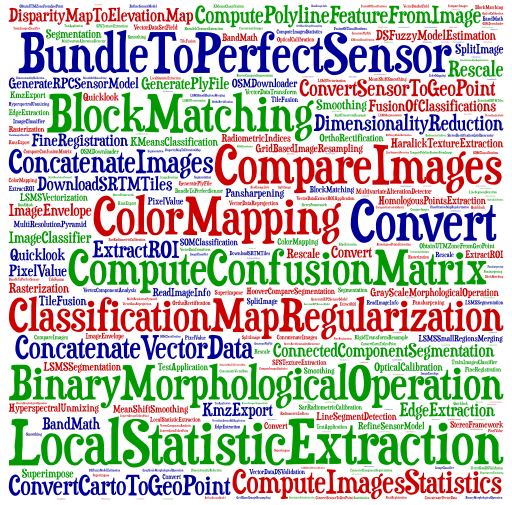
\includegraphics[width=\textwidth]{images/cloud_applications.png}
\end{columns}
\end{frame}



\begin{frame}[fragile]
\frametitle{Applications: appel depuis la ligne de commande}
\begin{scriptsize}
\vspace{-0.5cm}\begin{verbatim}
$ otbcli_OrthoRectification

ERROR: Waiting for at least one parameter...
This is the OrthoRectification application, version 5.2.1
This application allows to ortho-rectify optical images from supported sensors.

Complete documentation: http://www.orfeo-toolbox.org/Applications/OrthoRectification.html

Parameters:
        -progress                <boolean>        Report progress
MISSING -io.in                   <string>         Input Image  (mandatory)
MISSING -io.out                  <string> [pixel] Output Image  [pixel=uint8/uint16/int16/uint32/int32/float/double] (default value is float) (mandatory)
        -map                     <string>         Output Cartographic Map Projection [utm/lambert2/lambert93/wgs/epsg] (mandatory, default value is utm)
        -map.utm.zone            <int32>          Zone number  (mandatory, default value is 31)
        -map.utm.northhem        <boolean>        Northern Hemisphere  (optional, off by default)
        -map.epsg.code           <int32>          EPSG Code  (mandatory, default value is 4326)
        -outputs.mode            <string>         Parameters estimation modes [auto/autosize/autospacing/outputroi/orthofit] (mandatory, default value is auto)
MISSING -outputs.ulx             <float>          Upper Left X  (mandatory)
MISSING -outputs.uly             <float>          Upper Left Y  (mandatory)
MISSING -outputs.sizex           <int32>          Size X  (mandatory)
MISSING -outputs.sizey           <int32>          Size Y  (mandatory)
MISSING -outputs.spacingx        <float>          Pixel Size X  (mandatory)
MISSING -outputs.spacingy        <float>          Pixel Size Y  (mandatory)
        -outputs.lrx             <float>          Lower right X  (optional, off by default)
        -outputs.lry             <float>          Lower right Y  (optional, off by default)
        -outputs.ortho           <string>         Model ortho-image  (optional, off by default)
        -outputs.isotropic       <boolean>        Force isotropic spacing by default  (optional, on by default)
        -outputs.default         <float>          Default pixel value  (optional, on by default, default value is 0)
        -elev.dem                <string>         DEM directory  (optional, off by default)
        -elev.geoid              <string>         Geoid File  (optional, off by default)
        -elev.default            <float>          Default elevation  (mandatory, default value is 0)
        -interpolator            <string>         Interpolation [bco/nn/linear] (mandatory, default value is bco)
\end{verbatim}
\end{scriptsize}
\end{frame}

\begin{frame}[fragile]
\frametitle{Applications OTB: Interface graphique}
\begin{center}
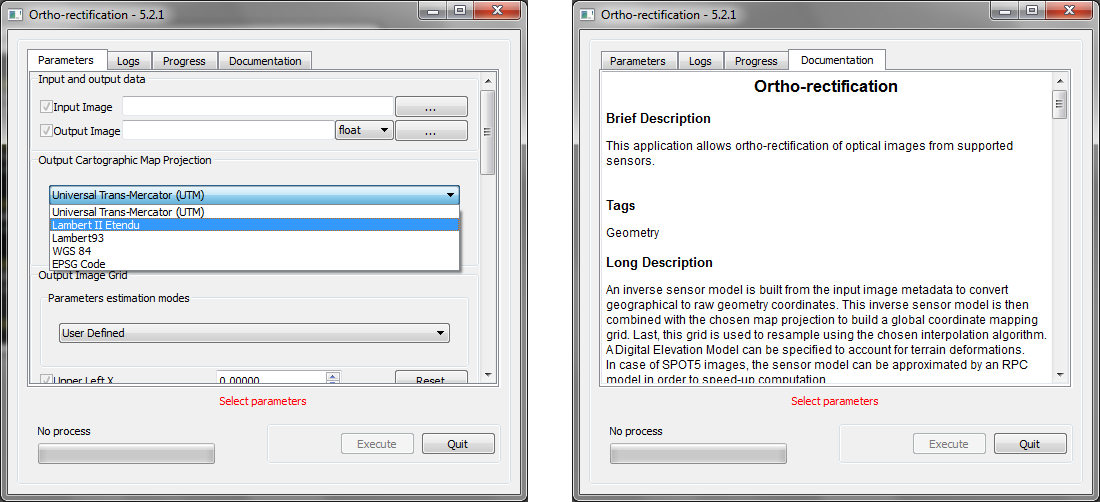
\includegraphics[width=1\textwidth]{images/otbgui.png}
\end{center}
\end{frame}

\begin{frame}[fragile]
\frametitle{Applications: appel depuis l'interface Python}
\begin{lstlisting}[language=python,breaklines=true,breakatwhitespace=true,frame = tb,framerule = 0.25pt,fontadjust,backgroundcolor={\color{listlightgray}},basicstyle = {\ttfamily\tiny},keywordstyle = {\ttfamily\color{listkeyword}\textbf},identifierstyle = {\ttfamily},commentstyle = {\ttfamily\color{listcomment}\textit},stringstyle = {\ttfamily},showstringspaces = false,showtabs = false,numbers = none,numbersep = 6pt, numberstyle={\ttfamily\color{listnumbers}},tabsize = 2]
#!/usr/bin/python

# Import the otb applications package
import otbApplication

# The following line creates an instance of the OrthoRectification application
OrthoRectification = otb.Registry.CreateApplication("OrthoRectification")

# The following lines set all the application parameters:
OrthoRectification.IO.IN = "QB_TOULOUSE_MUL_Extract_500_500.tif"
OrthoRectification.IO.OUT = "QB_Toulouse_ortho.tif"

app.MAP = 'epsg'
app.MAP.EPSG.CODE = 32768

# The following line execute the application
OrthoRectification.ExecuteAndWriteOutput()
\end{lstlisting}
\end{frame}


\begin{frame}
\frametitle{Monteverdi (accès aux applications OTB)}
\begin{minipage}[t][6cm][t]{\textwidth}
\begin{center}
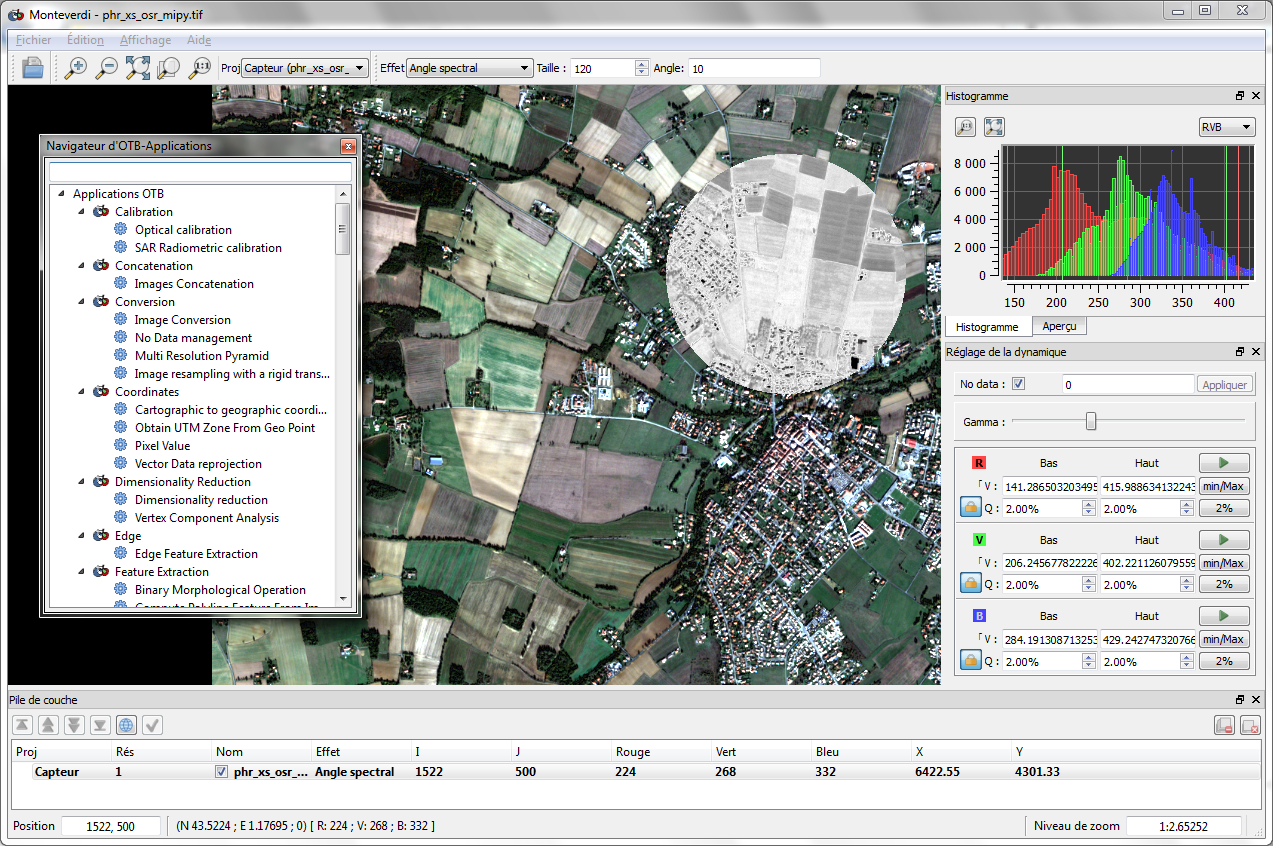
\includegraphics[width=1.0\textwidth]{images/monteverdi.png}
\end{center}
\end{minipage}
\end{frame}

%\vspace*{-3.0mm}
\begin{frame}
  \frametitle{QGIS (accès aux applications OTB)}
\begin{minipage}[t][6cm][t]{\textwidth}
\begin{center}
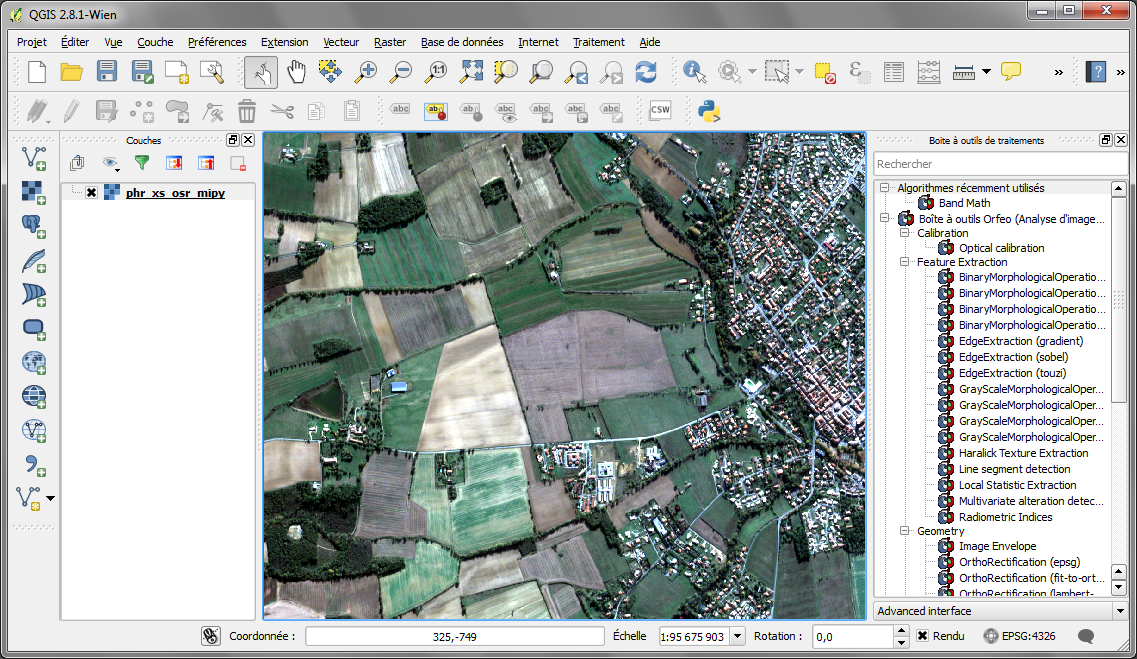
\includegraphics[width=1\textwidth]{images/otb_in_qgis.png}
\end{center}
\end{minipage}
\end{frame}

\begin{frame}
  \frametitle{Applications OTB ``as a service'' avec ZOO Project WPS}
\begin{minipage}[t][6cm][t]{\textwidth}
\begin{center}
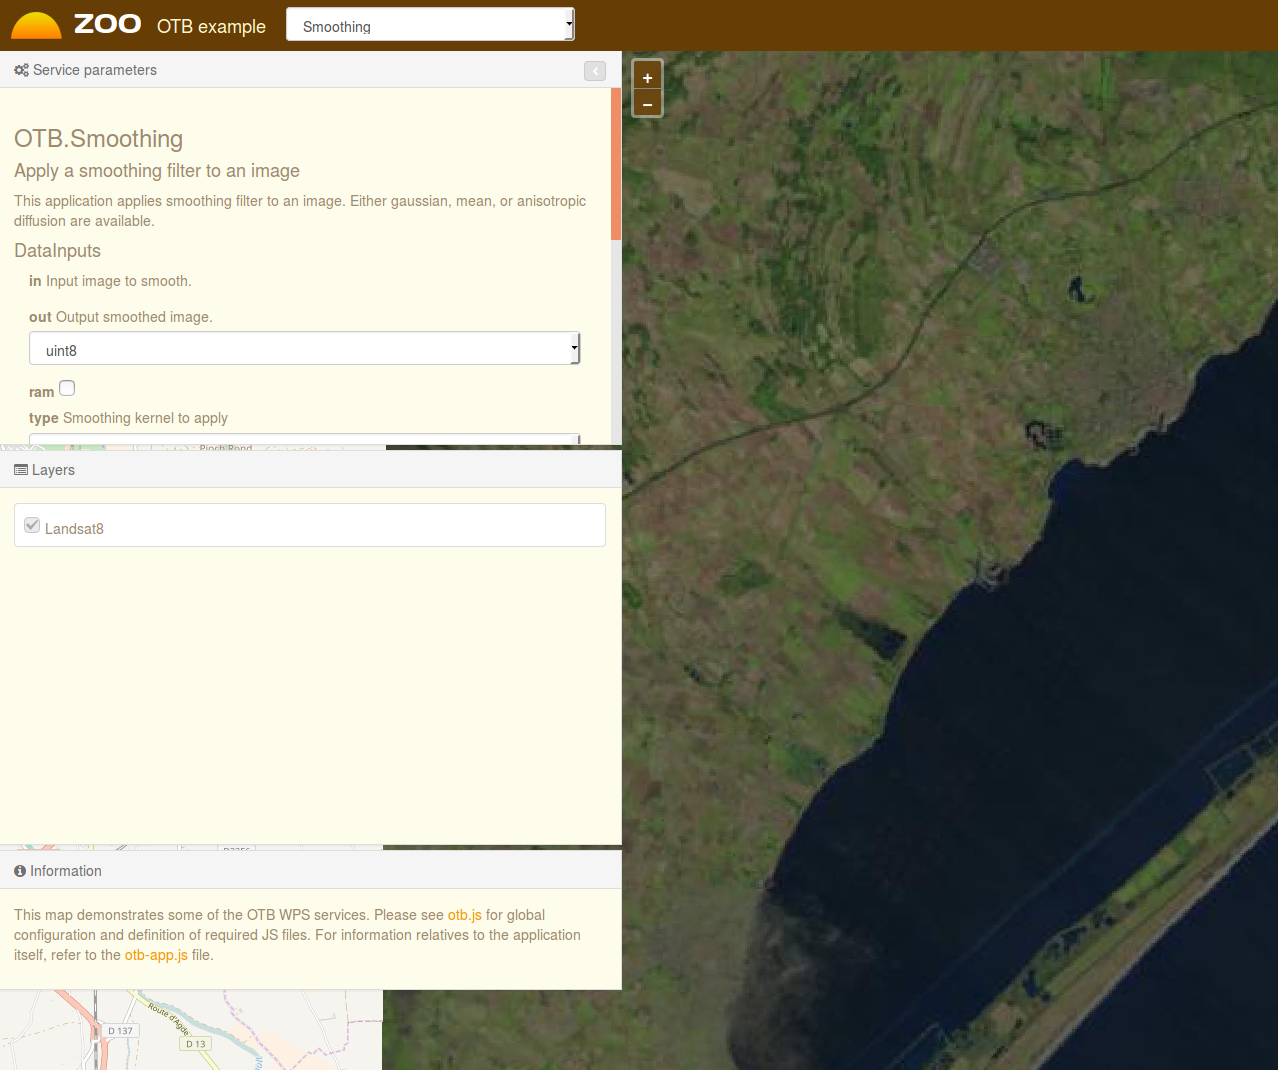
\includegraphics[width=0.7\textwidth]{images/otb_in_zoo.png}
\end{center}
\end{minipage}
\end{frame}

\section{Quoi de neuf dans l'ORFEO ToolBox?}

\begin{frame}
  \frametitle{6.0 (mai 2017)}
  \begin{block}{OTB}
    \begin{itemize}
      \item Changement de licence pour Apache v2.0
      \item Support OpenCV 3.0
      \item Application pour deburst des produits Sentinel1 IW SLC
      \item Sélection des bandes par noms de fichier étendus
      \item Classification non-supervisée intégrée au framework
      \item Application pour profils morphologiques
      \item Application pour classer des vecteurs
      \item Nettoyage des fonctions dépréciées
    \end{itemize}
    \end{block}
\end{frame}

\begin{frame}
  \frametitle{OTB est un logiciel OSGeo!}
  \begin{block}{OSGeo incubation}
    \begin{itemize}
      \item Processus formel pour intégrer de nouveaux logiciels avec le``label'' OSGeo
      \item Incubation de l'OTB a débuté en 2011
      \item Long voyage semé d'embûches...
    \end{itemize}
  \end{block}
  \begin{center}
  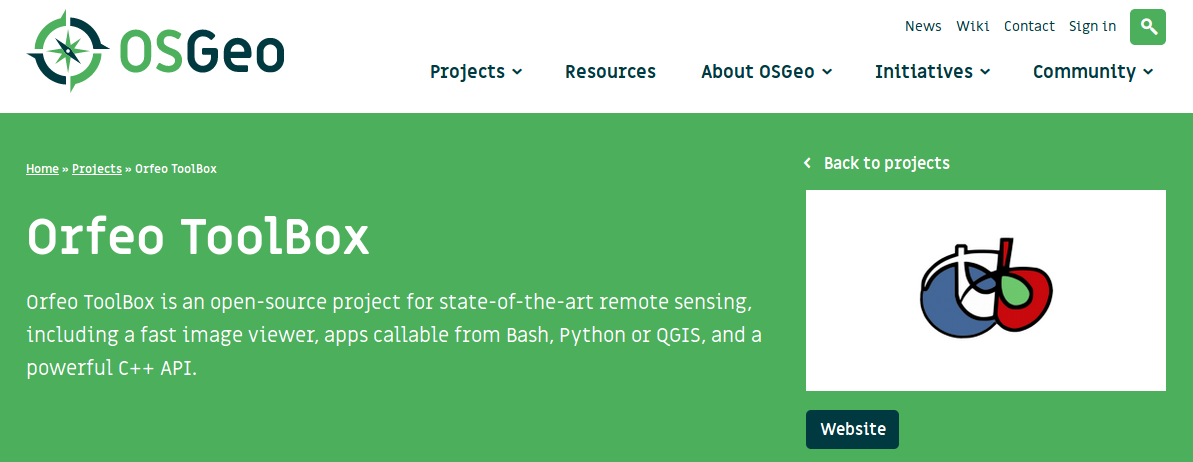
\includegraphics[width=0.35\textwidth]{images/osgeo-otb-website.png}
  \end{center}
  \begin{block}{L'âge de la maturité}
    \begin{itemize}
      \item Suivi les recommandations de l'OSGeo (gouvernance ouverte...)
      \item Processus qui a aidé l'OTB à ``grandir''
      \item Merci à l'OSGeo et à tous ses membres.
    \end{itemize}
  \end{block}
  
\end{frame}

\begin{frame}
  \frametitle{6.4 (Janvier 2018)}
  \begin{itemize}
  \item Améliorations du widget de sélection des fichiers multiples
  \item Application et filtre pour l'amélioration du contraste local (CLAHE)
  \item Amélioration du modèle générique de capteur SAR
  \item Support de Python 3
  \item Après cette release: déménagement vers \href{https://gitlab.orfeo-toolbox.org}{GitLab}!
  \end{itemize}
\end{frame}

%asuming you images are called "something-0.png" up to "something-11.png" 
\begin{frame}
  \frametitle{New in OTB 6.4: Contrast Enhancement - For fun and profit}
  \transduration<0-1>{0}
  \multiinclude[<+->][format=png, graphics={width=\textwidth}]{images/animation-clahe}
\end{frame}
    
  
\begin{frame}
  \frametitle{GitLab: plus facile, plus intégré}
  \begin{columns}
    \column{0.4\textwidth}
    \begin{itemize}
    \item Request for comments, bugs, feature requests $\Rightarrow$ issues gitlab
    \item Toute modification passe par une Merge Request
    \item Revue de code facilitée, lien entre issues et Merge Request
    \item Démarche facilitée pour les contributeurs
    \item Hébergement possible pour les Remote Modules
    \end{itemize}
    \column{0.6\textwidth}
    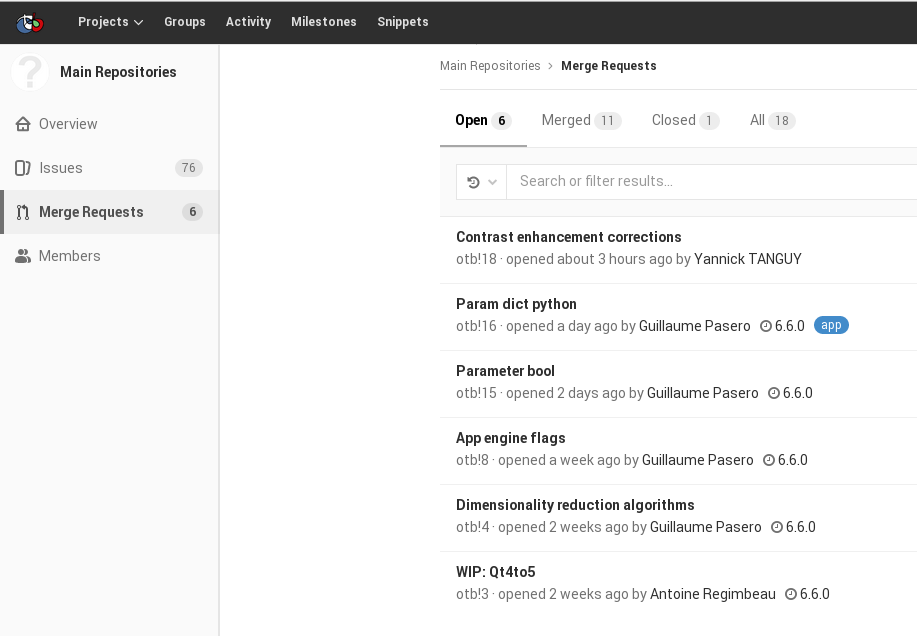
\includegraphics[width=\textwidth]{images/gitlab_mr.png}
    \end{columns}
\end{frame}


\section{Conclusion et perspectives}
\begin{frame}
\frametitle{Combien d'utilisateurs ?}
\begin{columns}[c]
\column{0.5\textwidth}
\begin{block}{Difficile à dire \ldots}
\begin{itemize}
    \item $\approx$ 600 membres sur la liste utilisateurs
    \item $\approx$ Entre 100 et 150 messages par mois
    \item $\approx$ 100 membres sur la liste développeurs
    \item $\approx$ 118 comptes sur le système de gestion des bugs
    \item $\approx$ 50 contributeurs (listé dans la documentation)
    \item $\approx$ 2000 téléchargements par mois pour l'installeur OTB (Win64)
  \end{itemize}
\end{block}
\begin{block}{Users Days 2015, 2016 et 2017}
  30 à 50 participants pendant 3 jours
\end{block}
\column{0.5\textwidth}
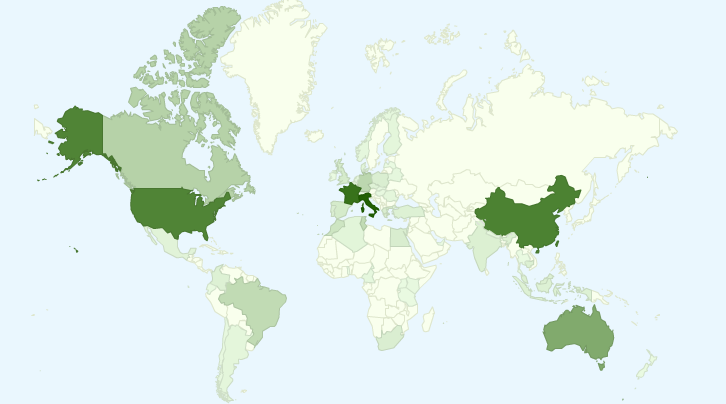
\includegraphics[width=0.9\textwidth]{images/OTB4_download_sourceforge_country_crop.png}\\
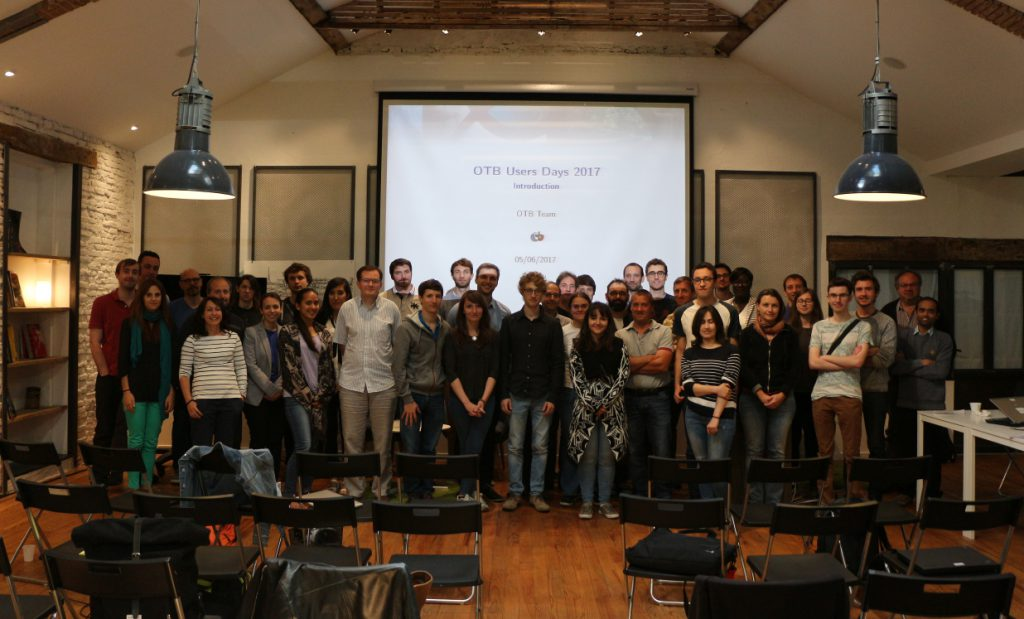
\includegraphics[width=0.9\textwidth]{images/userdays2017.jpg}
\end{columns}

\end{frame}


\section{Make OTB in QGIS Great Again}

\begin{frame}
\frametitle{2009: OTB-QGIS plugin (Archéologie)}
\begin{minipage}[t][6cm][t]{\textwidth}
\begin{center}
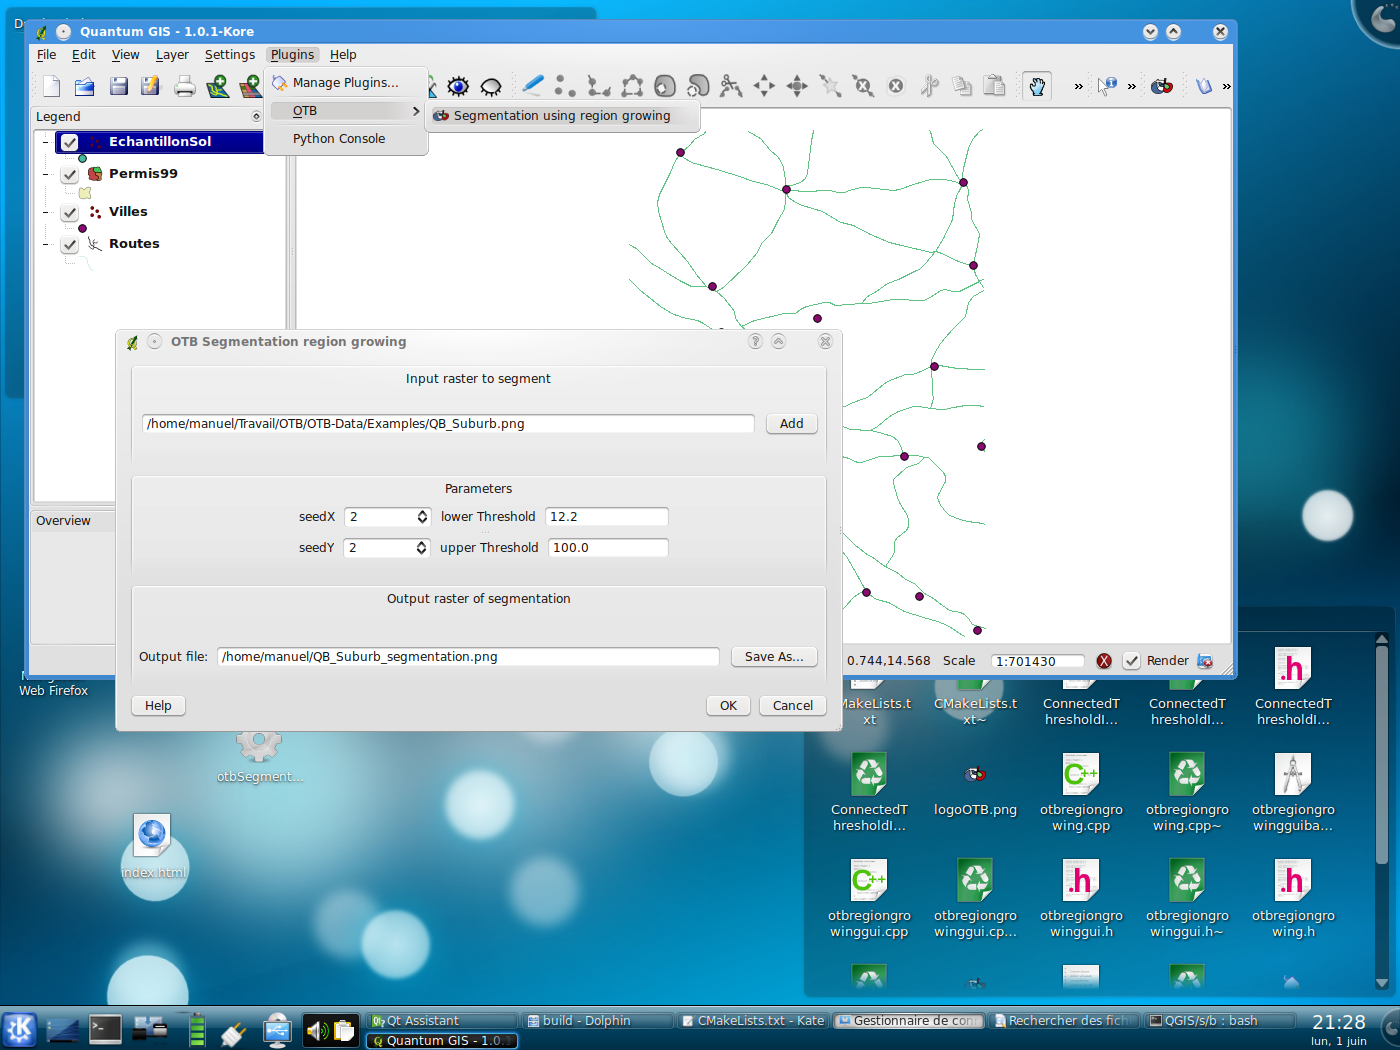
\includegraphics[width=0.7\textwidth]{images/otb-qgis-2009.png}
\end{center}
\end{minipage}
\end{frame}

\begin{frame}
\frametitle{2012-2017: OTB-QGIS disponible via le module processing}
\begin{minipage}[t][6cm][t]{\textwidth}
\begin{center}
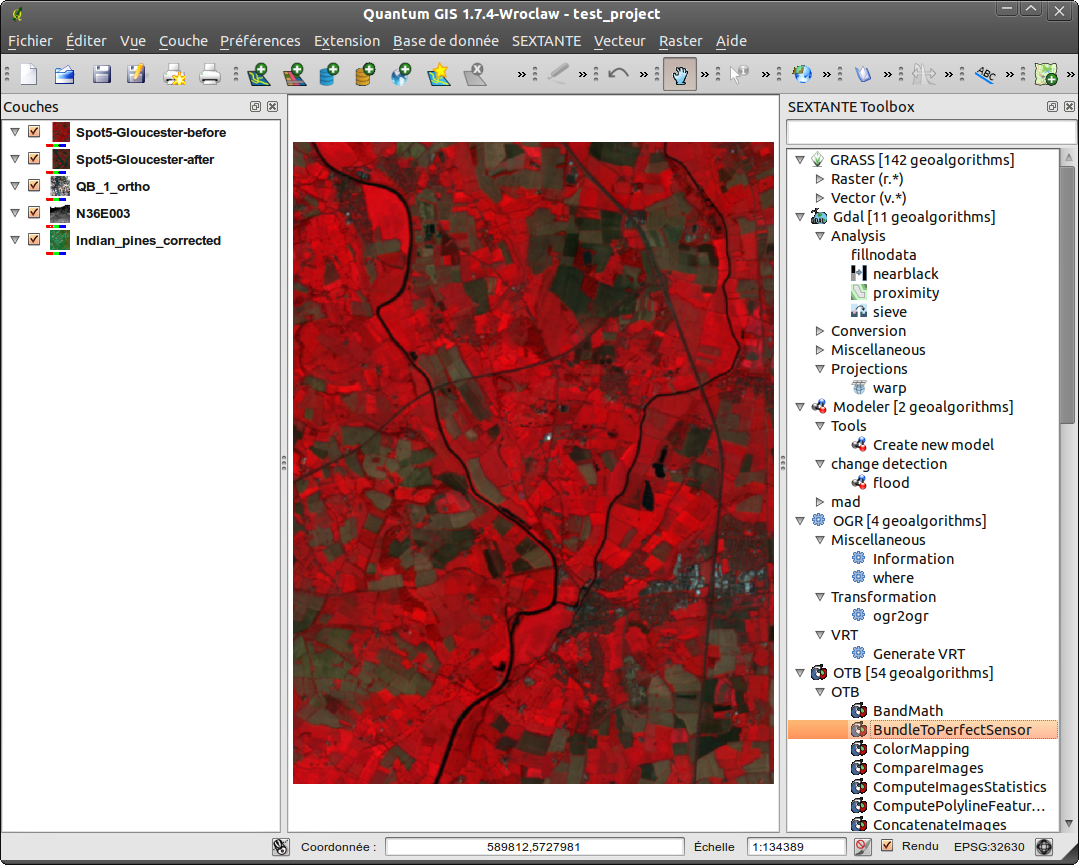
\includegraphics[width=0.7\textwidth]{images/otb_qgis.png}
\end{center}
\end{minipage}
\end{frame}

\begin{frame}
\frametitle{Accès OTB dans QGIS: A powerful wedding}
\begin{itemize}
\item Facilite l'accès à l'OTB (QGIS is mainstream)
\item Profite de l'interface et des fonctionnalités de QGIS (OTB GUI...)
\item Intégration dans le module ``processing'' de QGIS (bactch, Python...)
\item Collaboration très positive avec la communauté QGIS
\item Support des développeurs QGIS
\item OSGeo \textit{power}
\item \href{https://www.youtube.com/watch?v=ufSQ2SgSIV4}{Démo}: \url{https://www.youtube.com/watch?v=ufSQ2SgSIV4}
\end{itemize}
\end{frame}

\begin{frame}
\frametitle{Mais aussi des problèmes...}
\begin{itemize}
\item ``Comment on installe la dernière version de l'OTB dans QGIS?''
\item ``Quelles versions de l'OTB fonctionnent avec quelles versions de QGIS?''
\item ``Pourquoi l'application de segmentation OTB n'apparaît pas dans le menu QGIS?''
\item ``Pourquoi les applications OTB n'ont pas le même nom dans QGIS?''
\item ``J'abandonne OTB dans QGIS, rien ne fonctionne...''
\item \alert{STOP!}
\item 2018: on va améliorer tout ça
%\item Maintenance, Maintenance, Maintenance...
%\item Each version of otb needs to update list of descriptor files
%\item XML files which are hard to maintain.
%\item requires to update a blacklist and whitelist documents to list app that cannot be included and can be included
%\item needs manual update of these xml + followup on pull request
%\item works only with limited version of OTB (Not last release, mostly behind 3-4 releases)
%\item Nobody want to work on it from otb and qgis side. maintained by CS team
%\item Some applications were grouped, depending on their parameters : BinaryMorphologicalOperation (Closing, Dilate, Erode, Opening)
%\item Add new parameter in ParameterMultipleExternalInput processing, to use it in FusionOfClassifications
\end{itemize}

\end{frame}

\begin{frame}
  \frametitle{2018: OTB-QGIS plugin - L'âge de la maturité}
  \begin{itemize}
    %\item Easy maintenance for both OTB team and QGIS team
  \item Keep It Simple
  \item Faciliter la maintenance des versions OTB (pour les équipes OTB et QGIS)
    %\item Descriptors are generated, distributed and maintained by OTB
  \item Binaires OTB: Support QGIS ``out of the box''
  \item Toutes les applications OTB sont disponibles dans QGIS (même nom, même documentation...)  
    %\item Out of box support for qgis via binary packages
    %\item Applications are not grouped.
    %\item Development took a turn due to some *non-technical*/politic issues in
    %qgis and otb
  \item \alert{Version bêta} disponible sous la forme d'un plugin
  \item Plugin sera prochainement ajouter aux sources de QGIS
    %\item Will be added back to QGIS processing core later (Thanks to QGIS team)
    %\item Support for remote modules
    %\item OTB processing provider knows to recreate descriptor file for apps (if not found)
    %\item \alert{Version beta} disponible sous la forme d'un plugin
    % First version is distributed a plugin
  \item
    \href{https://gitlab.orfeo-toolbox.org/orfeotoolbox/qgis-otb-plugin}{https://gitlab.orfeo-toolbox.org/orfeotoolbox/qgis-otb-plugin}{Source
      nouveau plugin}
  \item Sera compatible de QGIS 3.1 (prévu pour Juin 2018)
  \item Merci aux équipes QGIS!
  \end{itemize}
\end{frame}

\begin{frame}
\frametitle{Configuration provider OTB dans QGIS}
\begin{center}
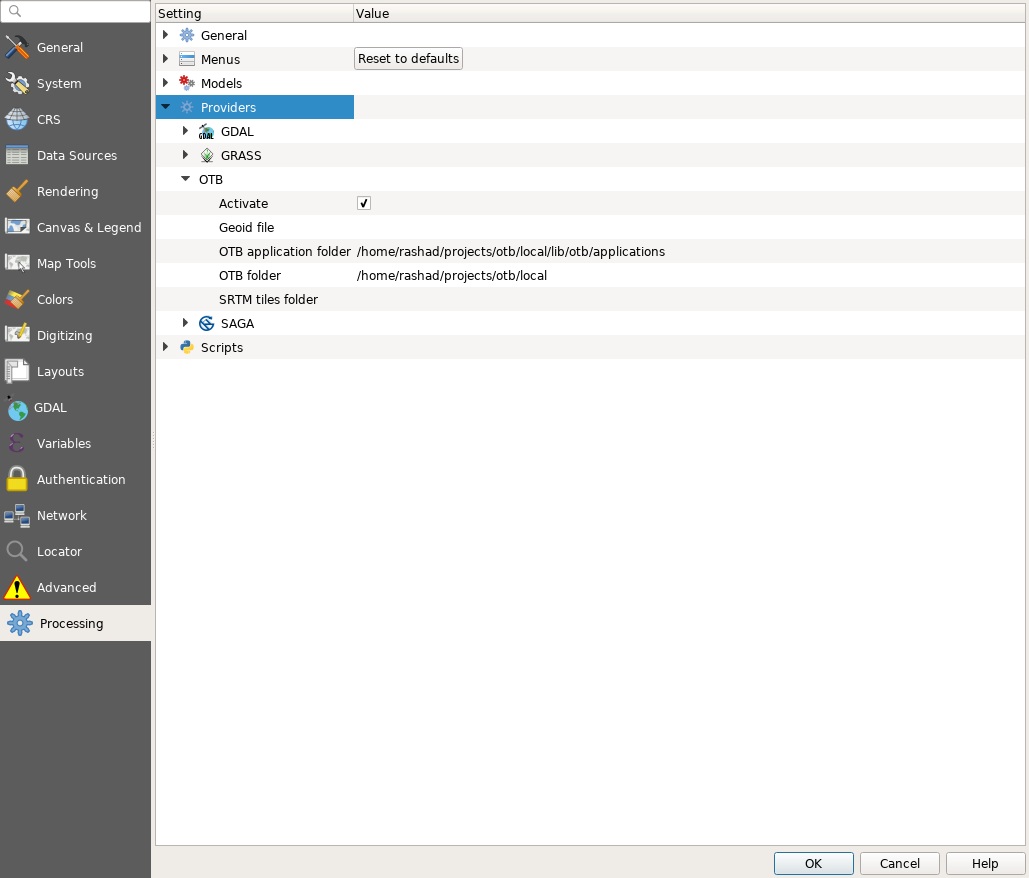
\includegraphics[width=0.8\textwidth]{images/qgis_otb_provider_config.png}
\end{center} 
\end{frame}

\begin{frame}
\frametitle{Interface de l'application \textit{Smoothing}}
\begin{center}
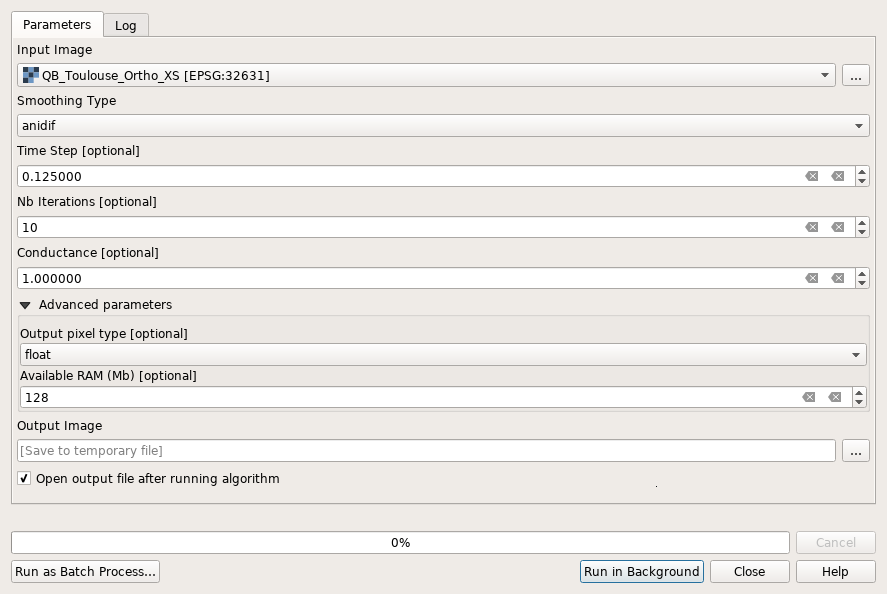
\includegraphics[width=0.8\textwidth]{images/qgis_smoothing.png}
\end{center} 
\end{frame}

\begin{frame}
\frametitle{Interface de l'application \textit{TrainImagesClassifier}}
\begin{center}
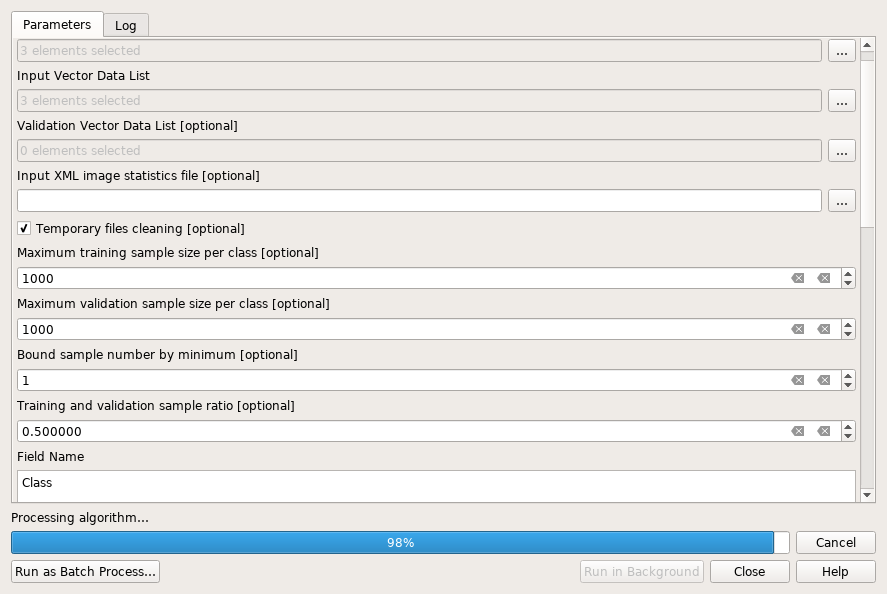
\includegraphics[width=0.8\textwidth]{images/qgis_train_classif.png}
\end{center} 
\end{frame}



\section{Conclusion}

\begin{frame}
\frametitle{Support/Aide/Contribution}
\vspace{-0.2cm}
\begin{block}{Ressources}
\vspace{-0.2cm}
\begin{description}
\item[Site web] \href{http://www.orfeo-toolbox.org}{orfeo-toolbox.org}
\item[Wiki] \href{http://wiki.orfeo-toolbox.org}{wiki.orfeo-toolbox.org}
\item[Blog] \href{http://blog.orfeo-toolbox.org}{blog.orfeo-toolbox.org}
\end{description}
\end{block}
\vspace{-0.2cm}
\begin{block}{Documentation et aide}
\vspace{-0.2cm}
\begin{description}
\item[Doxygen] \href{http://www.orfeo-toolbox.org/doxygen/}{doxygen}
\item[Documentation] Software Guide et CookBook (remote sensing recipes)
\item[Liste de diffusion utilisateurs] otb-users@googlegroups.com
\item[Liste de diffusion développeurs] otb-developers@googlegroups.com
\end{description}
\end{block}
\vspace{-0.2cm}
\begin{block}{Follow-up}
\vspace{-0.2cm}
\begin{description}
\item[Code, bugs, contributions, feature requests \ldots] \href{https://gitlab.orfeo-toolbox.org/orfeotoolbox/otb}{gitlab.orfeo-toolbox.org}
\item[Météo?] \href{http://dash.orfeo-toolbox.org}{dash.orfeo-toolbox.org}
\end{description}
\end{block}
\end{frame}

\begin{frame}
  \frametitle{Journée des Utilisateurs OTB 2018 - Montpellier - 19/10/2018}
  \begin{description}
  \item[Où?] \href{http://www.agropolis.fr/pratique/locaux.php}{Agropolis International}
  \item[Quand?] 19 Octobre 2018 - Suite séminaire \href{http://theia2018.sciencesconf.org}{THEIA}
  \item[Quoi?] Présentations, retour d'expérience, formations, tutoriels...
  \item[Comment?] Gratuit, ouvert à tous et à toutes!
  \item[Je m'inscris!] \url{https://tinyurl.com/y7yzjvad}
  \end{description}
  \begin{center}
    \alert{Venez nombreux!}
  \end{center}
  \begin{center}
    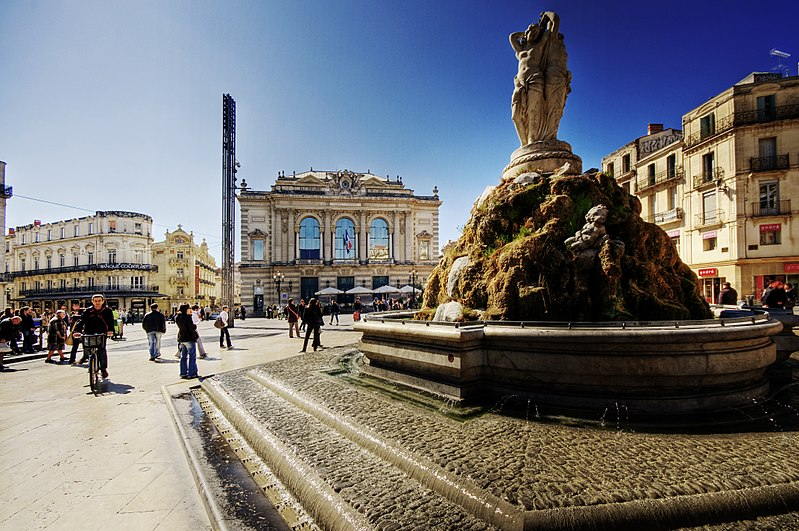
\includegraphics[width=0.45\textwidth]{images/montpellier.jpg}
  \end{center}

  
\end{frame}
  
\begin{frame}
\frametitle{Merci pour votre attention. Des questions?}
\begin{minipage}[t][6cm][t]{\textwidth}
\begin{center}
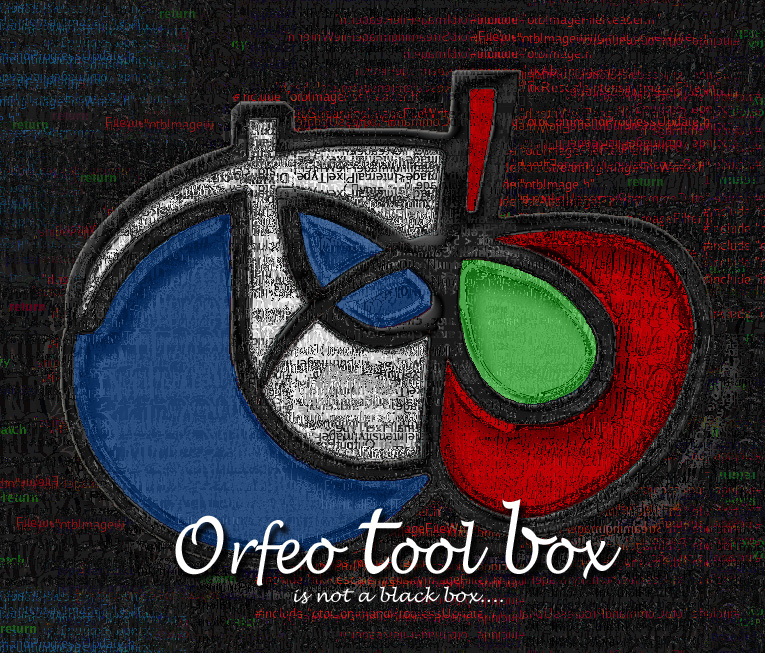
\includegraphics[width=0.65\textwidth]{images/LOGOTB_blackbox.png}
\end{center}
\end{minipage}
\end{frame}

\end{document}
